\begin{document}

\chapter{Results and Discussion}
\label{results}
Diachronic embeddings, which are trained for the purpose of tracing the change of word representations in vector space models, are met with challenges regarding how the training is evaluated. In this study, the trained embeddings are first examined in an interactive interface in order to explore the structure of the diachronic embeddings in general. Furthermore, the analogical reasoning task and the bootstrapping method are employed as an attempt to pinpoint the properties of the embeddings that might be influenced by the source data, or digitalized ancient texts to be specific. It is also worth noting that the evaluation and the discussions are complementary, for the ``bias'' in an embedding is also interpreted as a ``feature'', not only a ``bug'' \parencite{wevers2020digital}.

\section{Collocational-based Approach}
\label{results_collocational}
The results of the \gls{vnc} periodization are plotted as dendrograms in \fref{fig:collogram_VNC}, and the tables of collograms with the highest association scores are provided in \ref{appendix:pre_collograms}, and \ref{appendix:post_collograms}, \ref{appendix:all_collograms} for pre-collograms, post-collograms, and all collograms irregardless of their positions to the keyword \jia\rspace. For example sentences with the collgrams, see \exref{sent:pre_collograms} and \exref{sent:post_collograms}.

In \fref{fig:collogram_VNC}, the correlation between the Qing dynasty and 1980s shows a drastically decreasing trend compared to that of its predecessor, the Ming dynasty and the Qing dynasty, marking a distinct new stage of development. Furthermore, the flattening of the line at 2 clusters in the scree plot in \fref{fig:collogram_screeplot} suggests no subgroups are identified. It is generalized from the results of the \gls{vnc} method that while modern Chinese is drastically different from pre-modern Chinese, the timeframe from the Tang dynasty to the Qing dynasty shows that each dynasty is dissimilar from one another and cannot be merged, even for the shortest dynasty Yuan.

\begin{figure}[H]
  \begin{subfigure}{0.3\textwidth}
    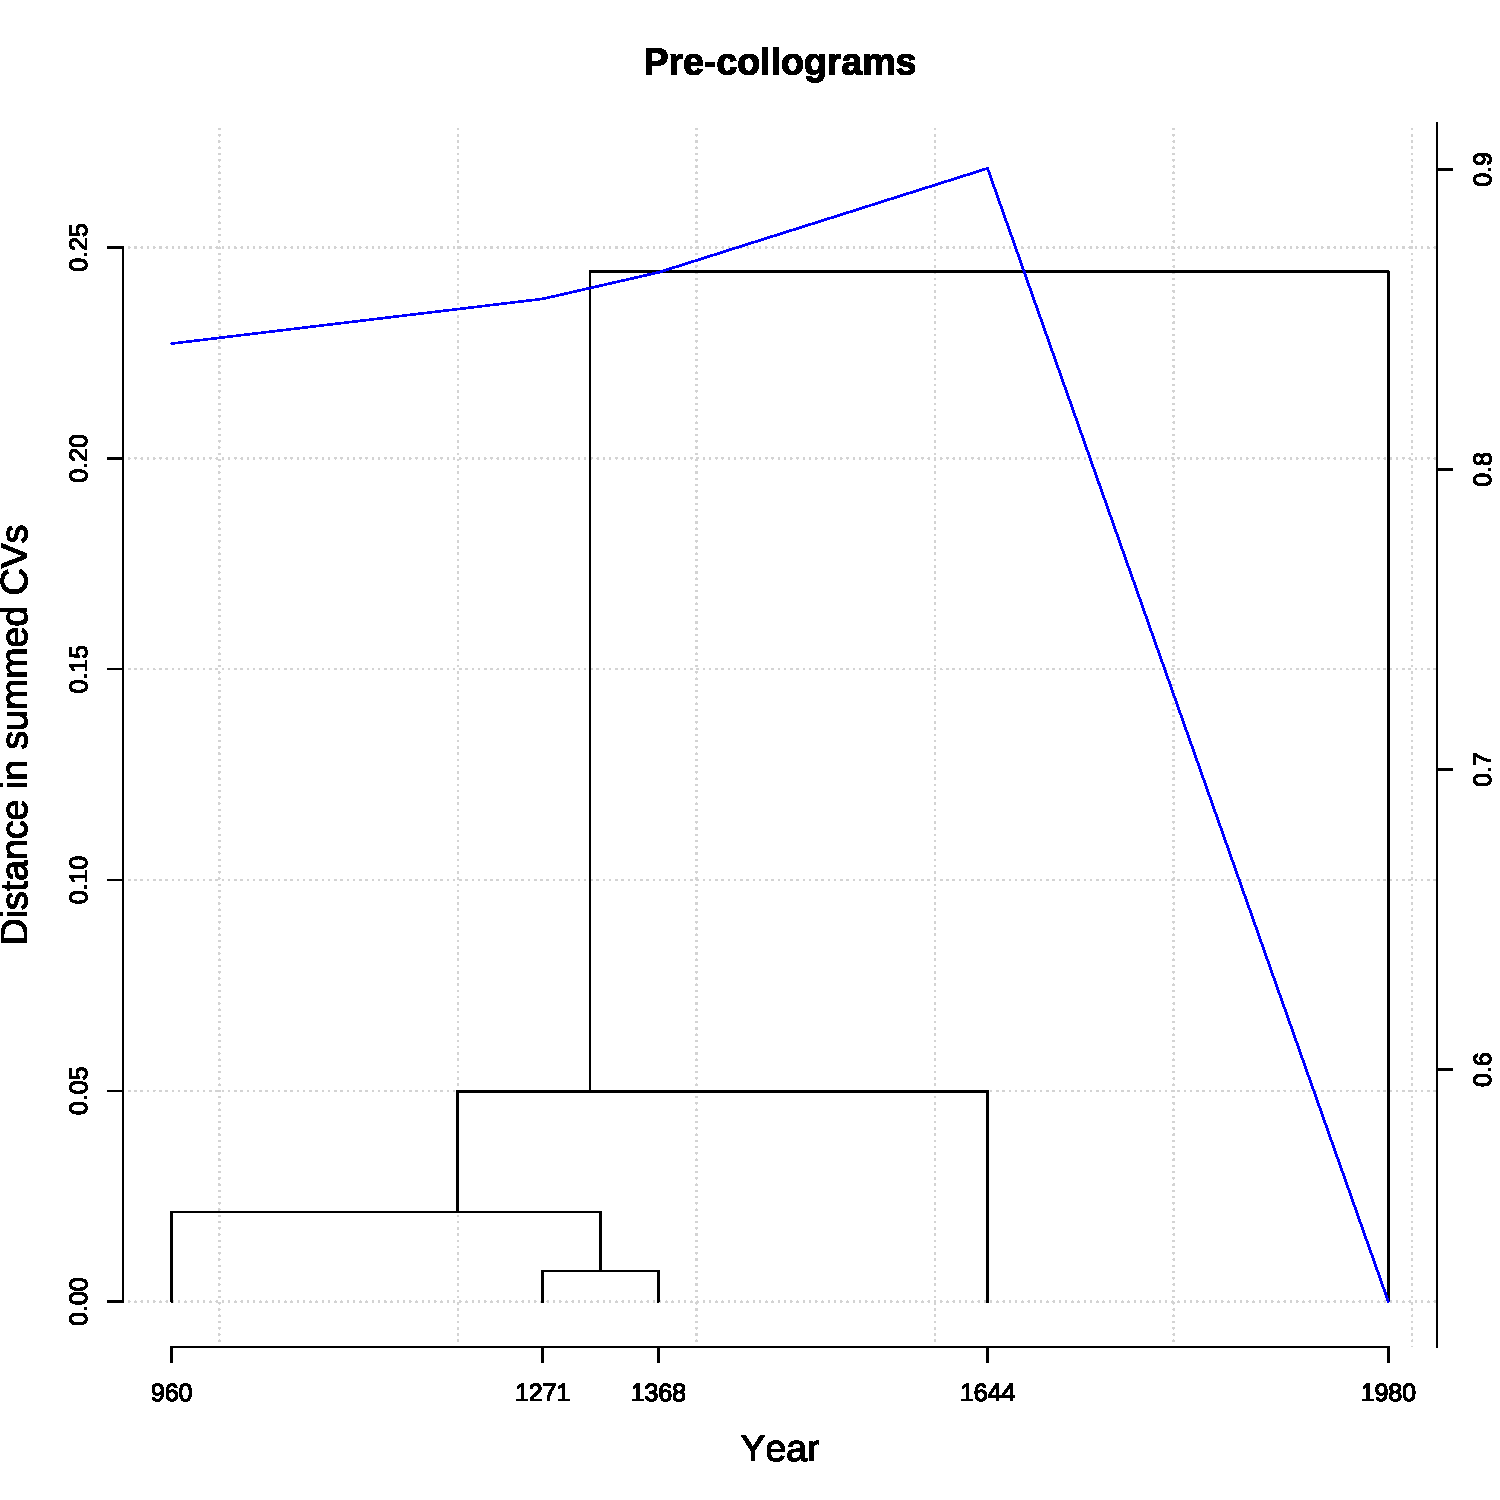
\includegraphics[width=\linewidth]{figures_new/VNC_lanbox/pre_collocate_df_VNC_cor.pdf}
    \caption{Pre-collograms}
  \end{subfigure}
  \quad
  \begin{subfigure}{0.3\textwidth}
    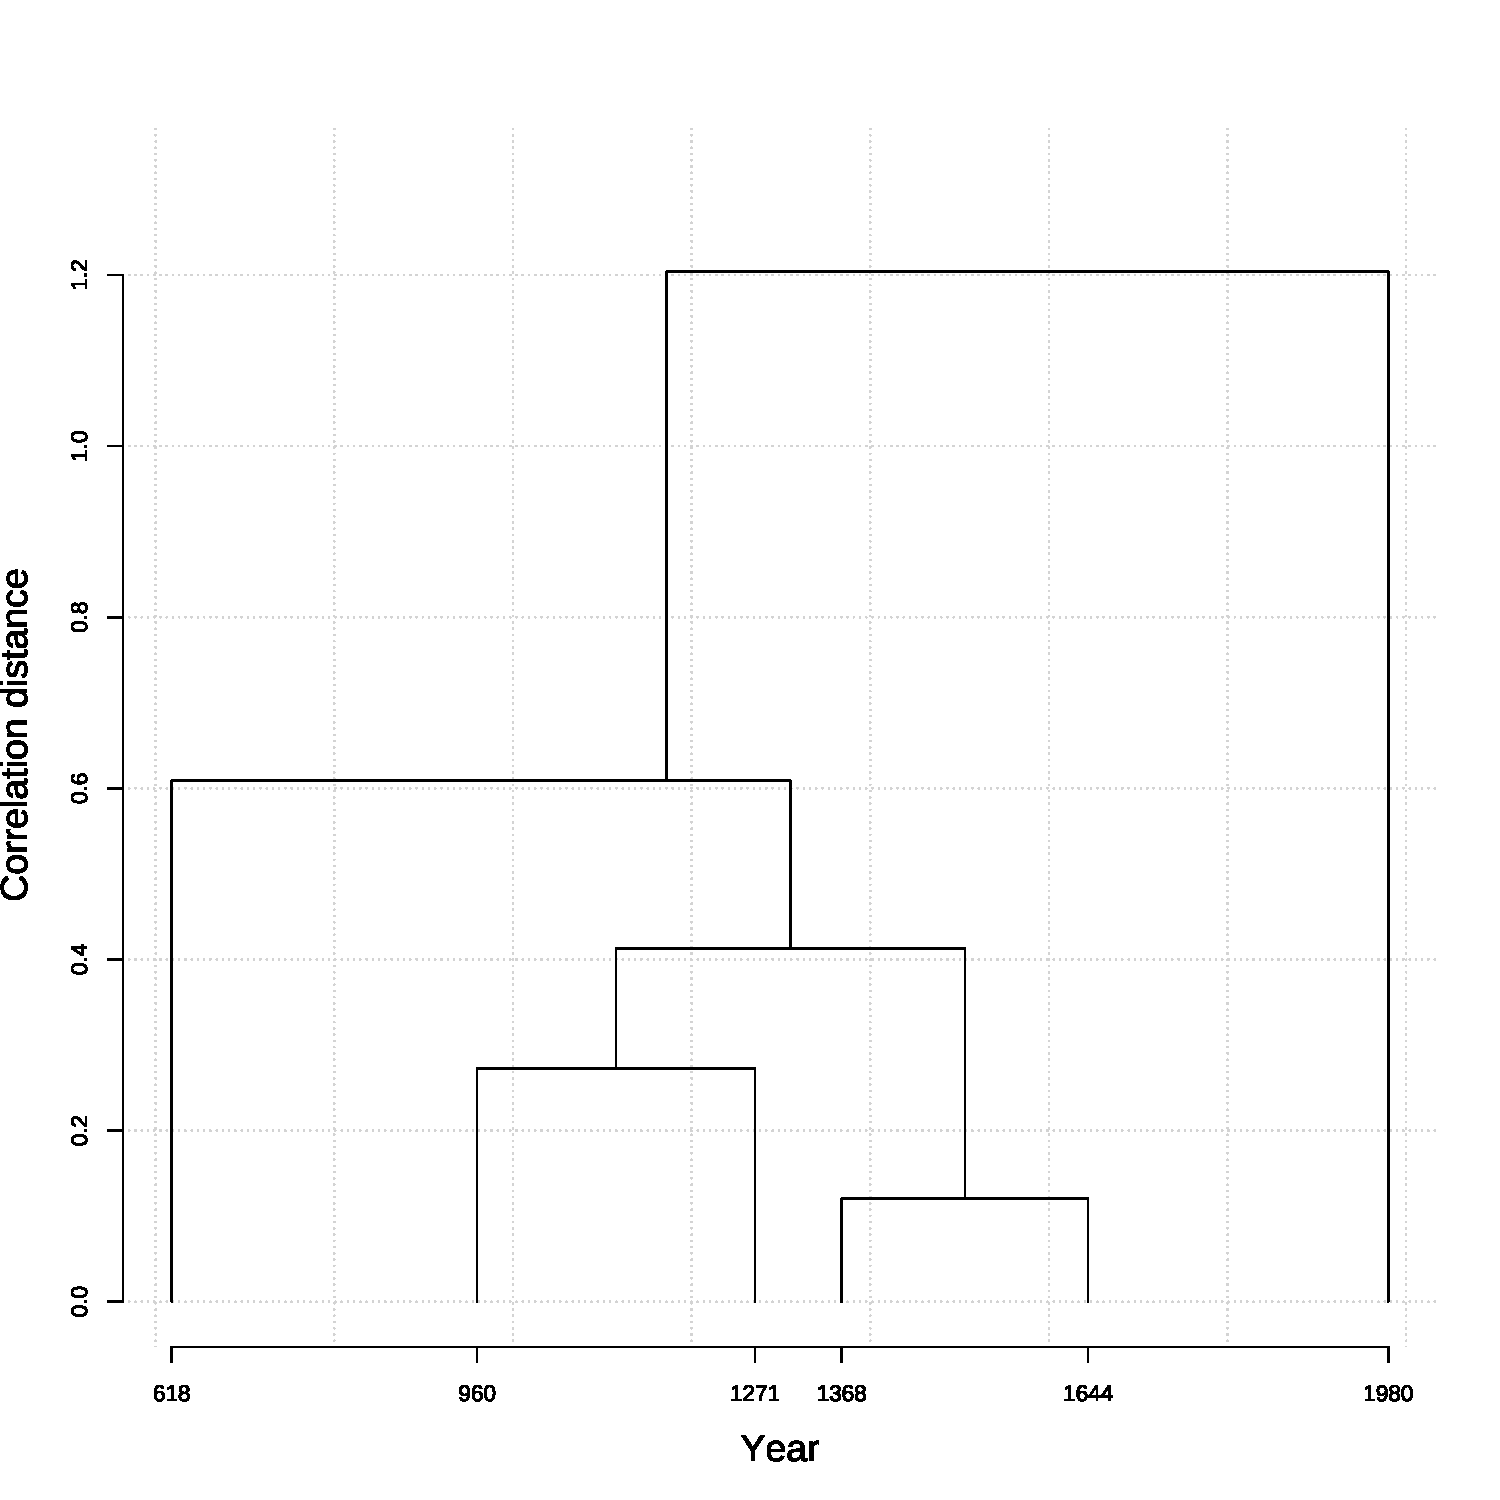
\includegraphics[width=\linewidth]{figures_new/VNC_lanbox/post_collocate_df_VNC_cor.pdf}
    \caption{Post-collograms}
  \end{subfigure}
  \quad
  \begin{subfigure}{0.3\textwidth}
    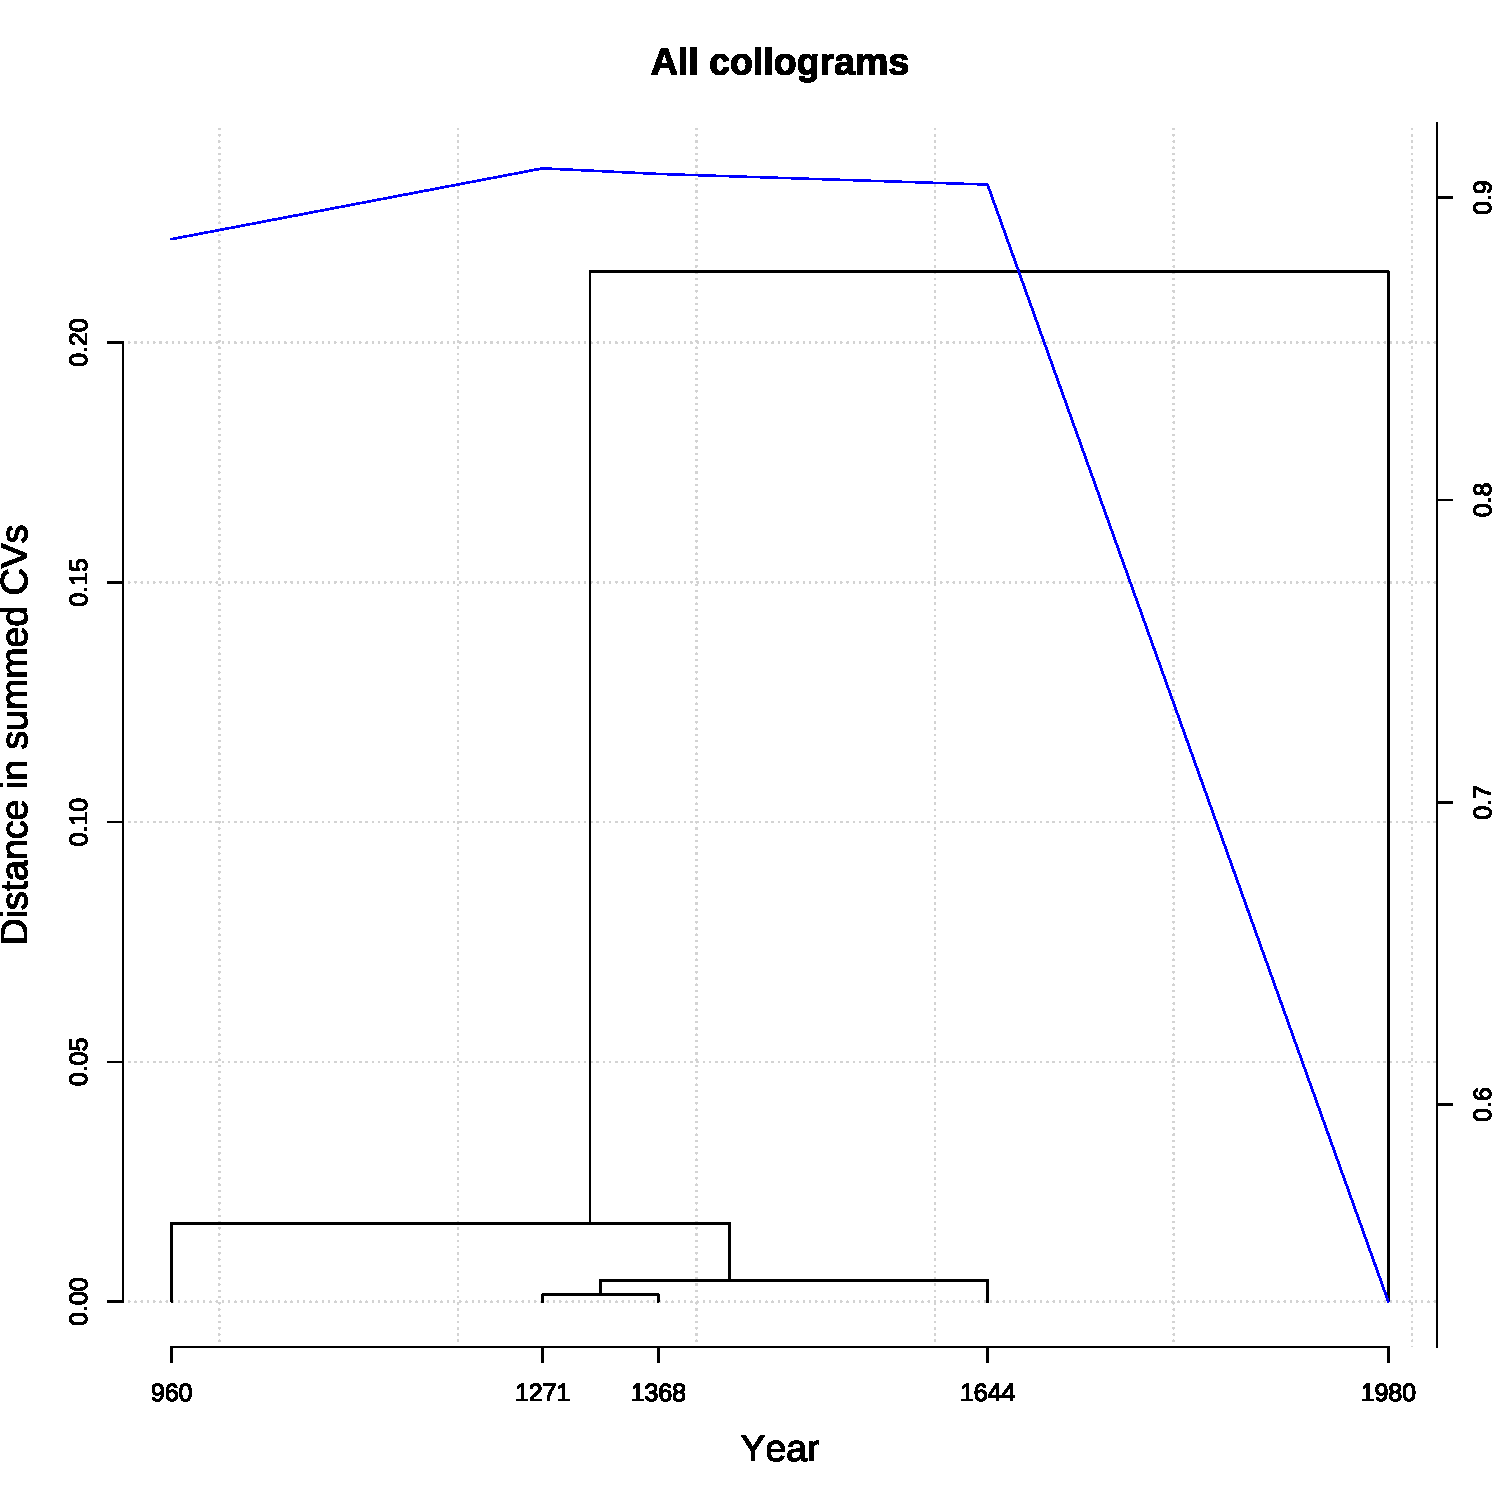
\includegraphics[width=\linewidth]{figures_new/VNC_lanbox/all_collocate_df_VNC_cor.pdf}
    \caption{All collograms}
  \end{subfigure}
  \caption{Results of VNC periodization of collograms before, after, and with \jia} \label{fig:collogram_VNC}
\end{figure}

\begin{figure}[H]
  \centering
  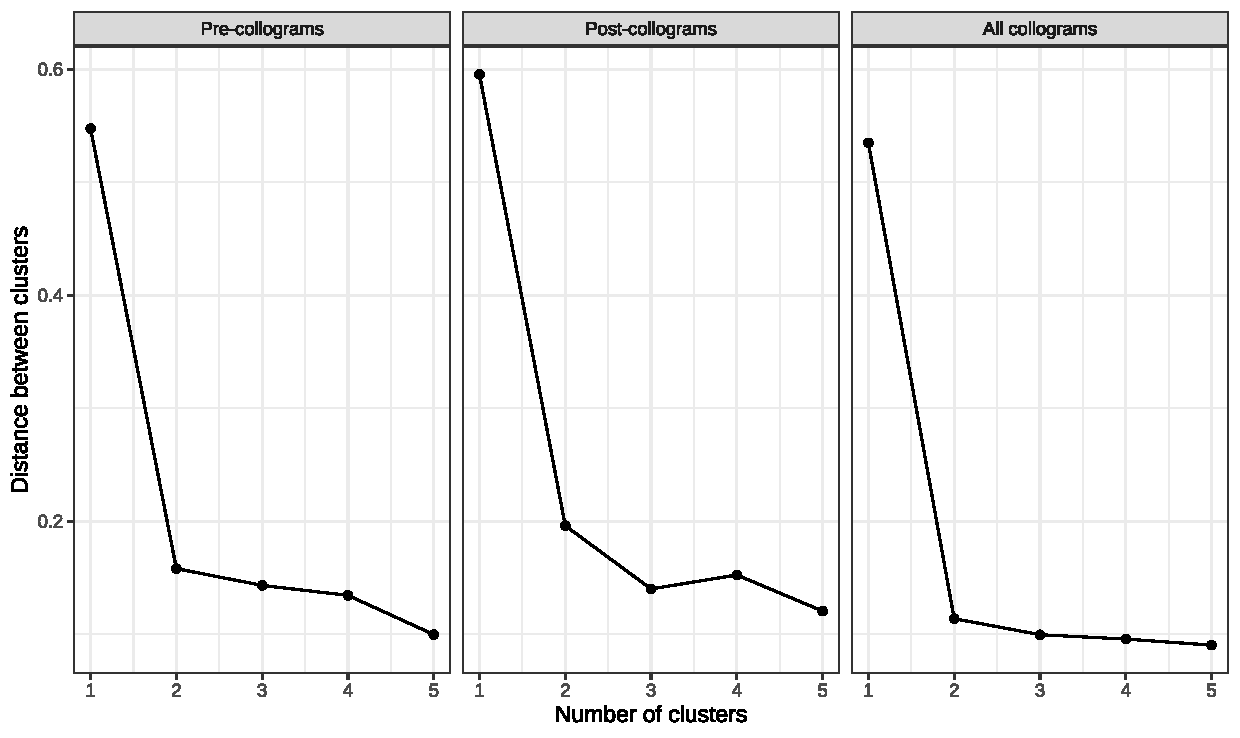
\includegraphics[width=0.75\textwidth,keepaspectratio]{figures_new/VNC_lanbox/screeplot_collocate.pdf}
  \caption{Screeplot for VNC periodization of collograms before, after, and with \jia} \label{fig:collogram_screeplot}
\end{figure}

\begin{exe}
  \ex{
    \begin{xlist}
      \ex{
        \sent{習侈難反故[世家]之能保者寡矣}%
        {Once one is accustomed to luxury, it is difficult to do otherwise. That's why it is rarely seen that fortune is passed down from the family lineage.}%
        {Ming}{恥言}
      }
      \ex{
        \sent{[國家]既遷河朔\ldots}%
        {The state's capital has moved to the northern bank of the Yellow River\ldots}%
        {Ming}{漕船志}
      }
    \end{xlist}
    \label{sent:pre_collograms}
  }
  \ex{
    \sent{[家語]云:與好人同行,如霧露中行,雖不濕衣,時時滋潤}%
    {As the Family Sayings states, ``Being surrounded with good people reminds you of walking in the dew; you won't be soaked to the skin, but take in the moisture from the air.''}%
    {Ming}{明心寶鑒}
    \label{sent:post_collograms}
  }
\end{exe}

\section{Word-level Embeddings}
\subsection{Evaluation on Analogical Reasoning}
Analogical thinking and context-dependent evidence lay a cognitive ground for the studies of semantic change \parencite{traugott2017semantic}. In terms of vector space models, analogical reasoning and similarity scoring are two tasks to intrinsically evaluate trained embeddings. Analogical reasoning is concerned with words in pairs or in groups because it is associated with the directionality of vectors that represent matched words. It is criticized, however, that common evaluation datasets mainly consist of geographical entities that would be non-existent in historical time periods \parencite{wevers2020digital,li2018analogical}. Despite its popularity, wide application, and the much effort into the expansion of datasets, the analogical reasoning task is not adaptable for diachronic or historical word embeddings \parencite{wevers2020digital}.

In this study, the training of word-level embeddings is examined based on the analogical reasoning task and the CA8 dataset. The CA8 dataset\footnote{\url{https://github.com/Embedding/Chinese-Word-Vectors}}, created by \textcite{li2018analogical}, is adopted to extract semantic relations in analogies, to the trained diachronic word-level embeddings in this study. While a variety of datasets and translated versions are available for the purpose of analogical reasoning, the CA8 dataset is characteristic of its attempt to not rely heavily on geographical names and proper nouns in the target analogical pairs. To mitigate the issues of named entities, 8 relational types are included. Additionally, among the \num{1307} analogical pairs in the type ``nature,'' \num{282} of them are single-character word pairs (or 1-gram, as labeled in the dataset), and the semantic relations are rich and elemental, including ``number, time, animal, plant, body, physics, weather, reverse, color'' \parencite{li2018analogical}. The availability of the CA8 dataset enables the possibility to extract the semantic relations in pre-modern Chinese texts in this study.

By solving the pair-based \sctext{3CosAdd} and \sctext{3CosMul} objectives \parencite{levy2014linguistic} proposed in \eref{equ:3cosadd} and \eref{equ:3cosmul}, it is found that \num{26} and \num{35} pairs are consistently identified across all time periods within smaller (window size set to 1) and larger (window size set to 10) window sizes. For example, pairs like 東-西:左-右 `east-west:left-right', 真-假:左-右 `real-fake: left-right', and 冷-熱:南-北 `cold-hot:south-north' are solved in all time periods, and the pair 冰-水:雪-雨 `ice-water:snow-rain' is also stably analogous except in the 1980s (For the results of solved coverages on the trained diachronic word-level embeddings, see \ref{appendix:analogical_reasoning}).

\begin{equation}
  b' = \arg\max_{d \in V}(\cos b', b - a + a'){,}
  \label{equ:3cosadd}
\end{equation}

\begin{equation*}
  where\: \cos(u,v) = \frac{u \cdot v}{\lVert{u}\rVert \cdot \lVert{v}\rVert}
\end{equation*}

\begin{equation}
  \arg\max_{b' \in V}\frac{\cos(b',b) \cos(b',a')}{\cos(b',a) + \varepsilon}{,}\: \varepsilon = 0.001
  \label{equ:3cosmul}
\end{equation}

However, it has not yet been feasible to extract semantic relations with set-based objectives like \sctext{3CosAvg}, for the mean of a set of vectors from the source and target single-character words under the same category defined in the dataset do not yield more analogical pairs in this study.

\subsection{Evaluation on Stability}
Following the evaluation of analogical reasoning for the diachronic word-level embeddings trained in the \sctext{fixed} settings, the evaluation for those trained in the \sctext{bootstrap} settings is performed to account for the variability resulting from document composition of different corpora. As shown in \fref{fig:stability_25}, the results show that the bootstrap samples become stable after 25 iterations, which echoes with the experiments conducted in \textcite{antoniak2018evaluating}.

\begin{figure}[H]
  \centering
  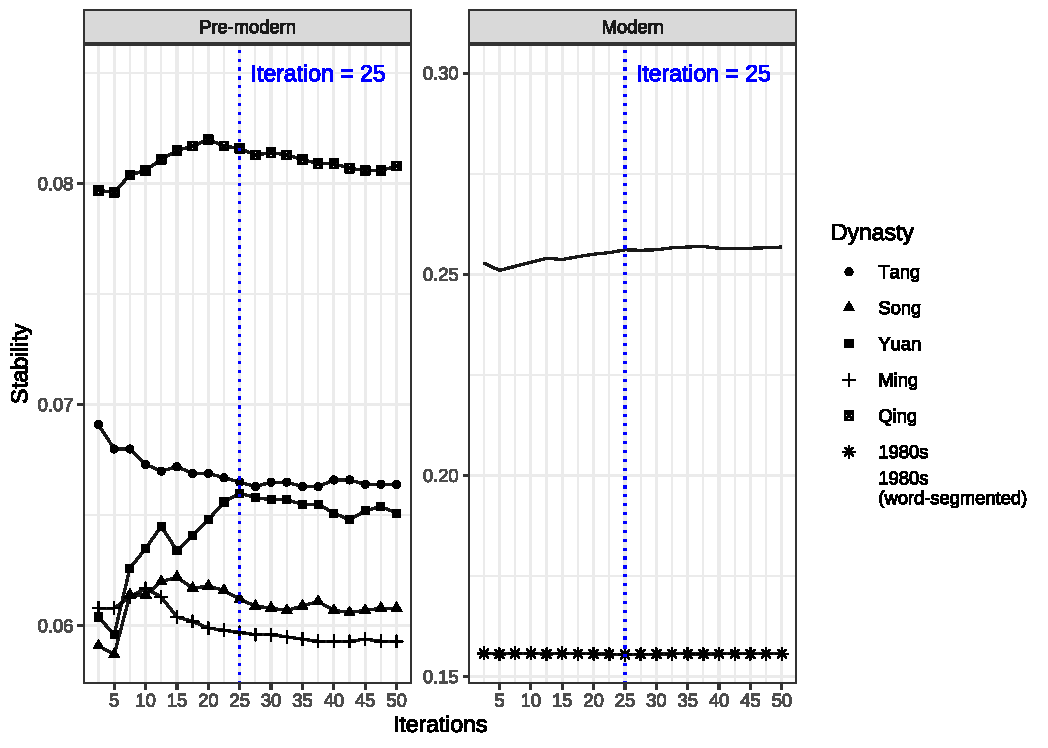
\includegraphics[width=0.95\textwidth,keepaspectratio]{figures_new/bootstrap_for_stability/stability.pdf}
  \caption{Mean stability over iterations based on query words extracted from LDA topic models and 20 nearest neighbors from \sctext{fixed} embeddings} \label{fig:stability_25}
\end{figure}

 Consequently, the analysis of nearest neighbors and their similarity scores can be compared between the \sctext{fixed} and \sctext{bootstrap} settings based on the 50 bootstrap samples. On top of that, the stability of nearest neighbors is evaluated with the number of top $N$ nearest neighbors set from 2 to 25, and the results are shown in \fref{fig:stability_jaccard}. The jaccard similarity scores suggest that it is appropriate to include at least 25 nearest neighbors to obtain a more homogeneous set of data.

\begin{figure}[H]
  \centering
  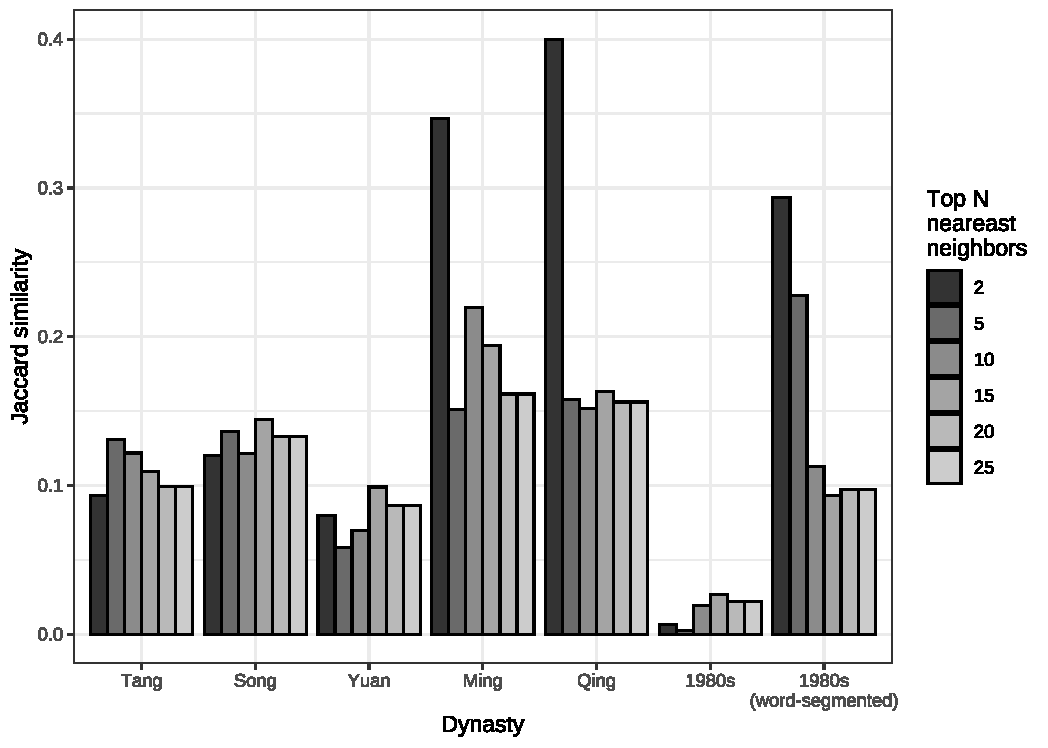
\includegraphics[width=0.85\textwidth,keepaspectratio]{figures_new/bootstrap_for_stability/jaccard_similarity_grey.pdf}
  \caption{Mean of Jaccard similarities from top $N$ nearest neighbors in the \sctext{bootstrap} settings. The higher the mean, the higher the degree of intersection for the nearest neighbors across the bootstrap iterations.} \label{fig:stability_jaccard}
\end{figure}

\subsection{Nearest neighbors of \jia}
The deployment of the trained diachronic word-level embeddings to Google's TensorBoard projector, a web-based interactive interface, is helpful to inspect all the datapoints and their metadata prior to the qualitative analysis of the keyword \jia in this study. The three-dimensional display of the training results offers a comprehensive overview of the datapoints that are originally structured in high-dimensional space. Figure~\ref{fig:tensorboard_PCA} and \fref{fig:tensorboard_tSNE} are the screenshots of the word-level diachronic embeddings from different angles. By filtering only the 6 datapoints that represent the keyword \jia from the Tang dynasty to the 1980s along with their neareast neighbors, the projector shows the results accordingly, as shown in \fref{fig:tensorboard_jia}.

\vspace*{\baselineskip}
\begin{figure}[H]
  \centering
  \begin{threeparttable}
  \begin{minipage}[b]{0.45\linewidth}
    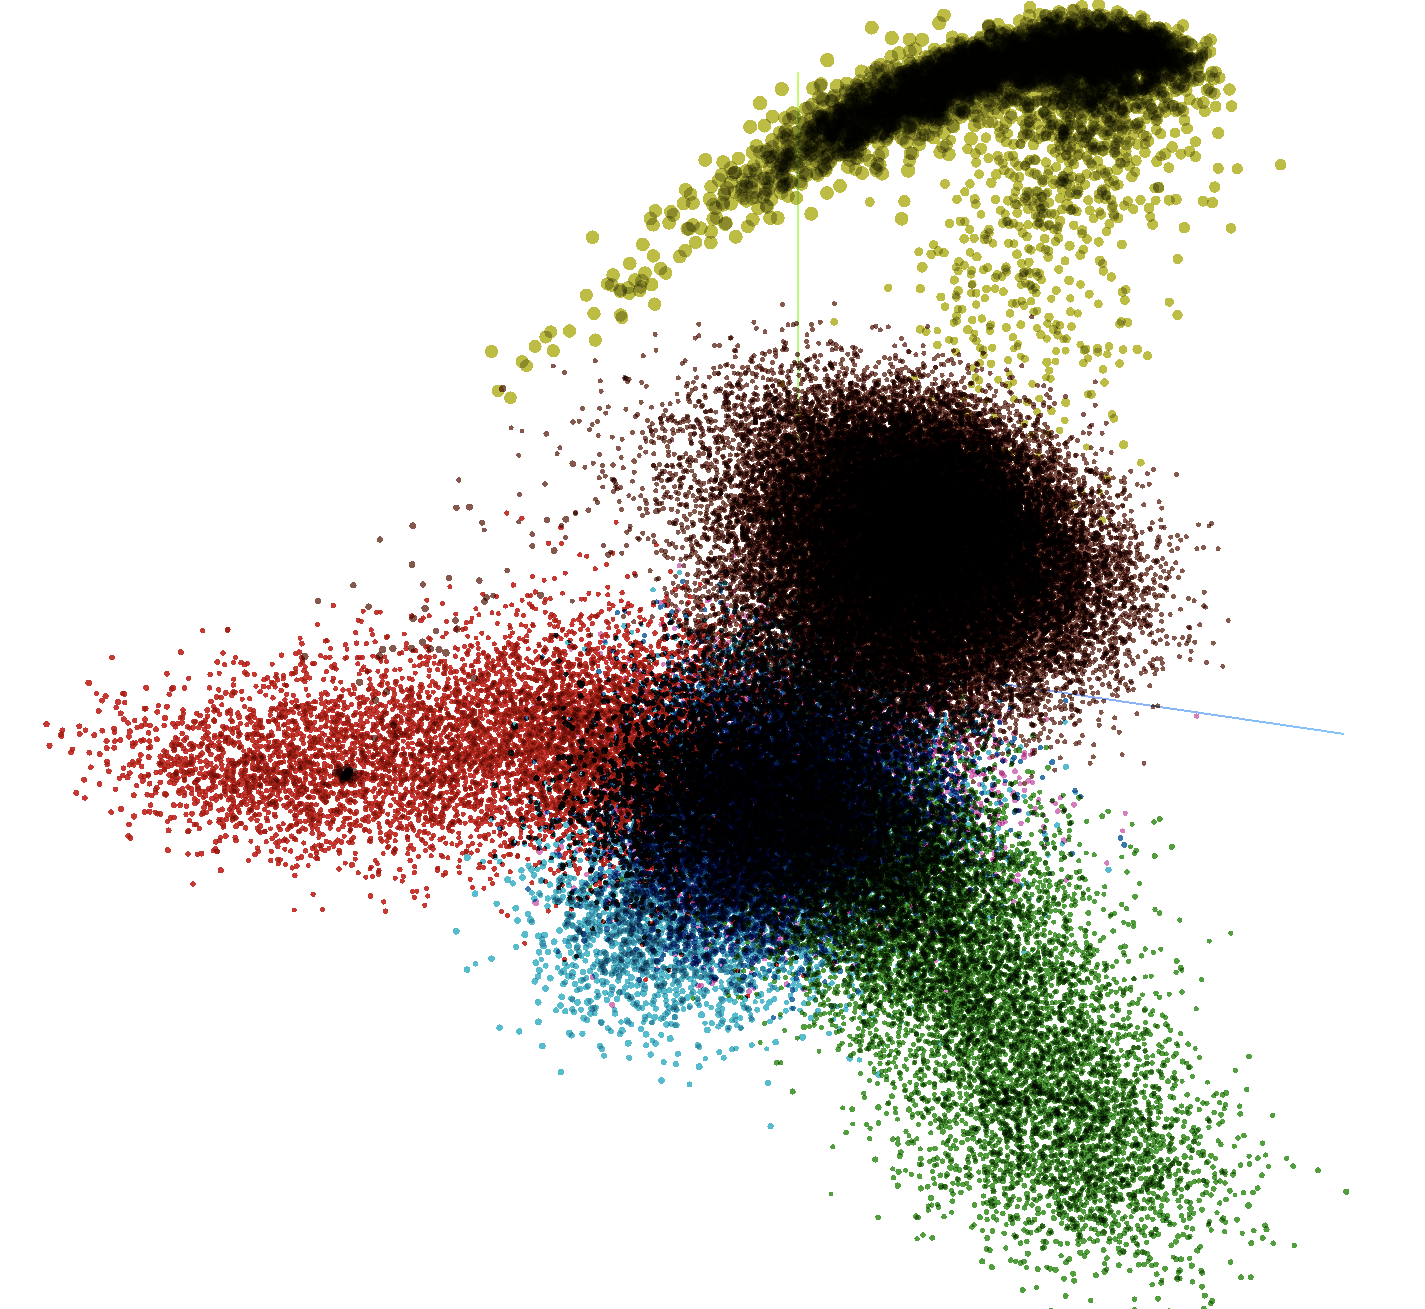
\includegraphics[width=\textwidth]{figures_new/from_old/pca_embedding_projector}
  \end{minipage}
  \quad
  \begin{minipage}[b]{0.45\linewidth}
    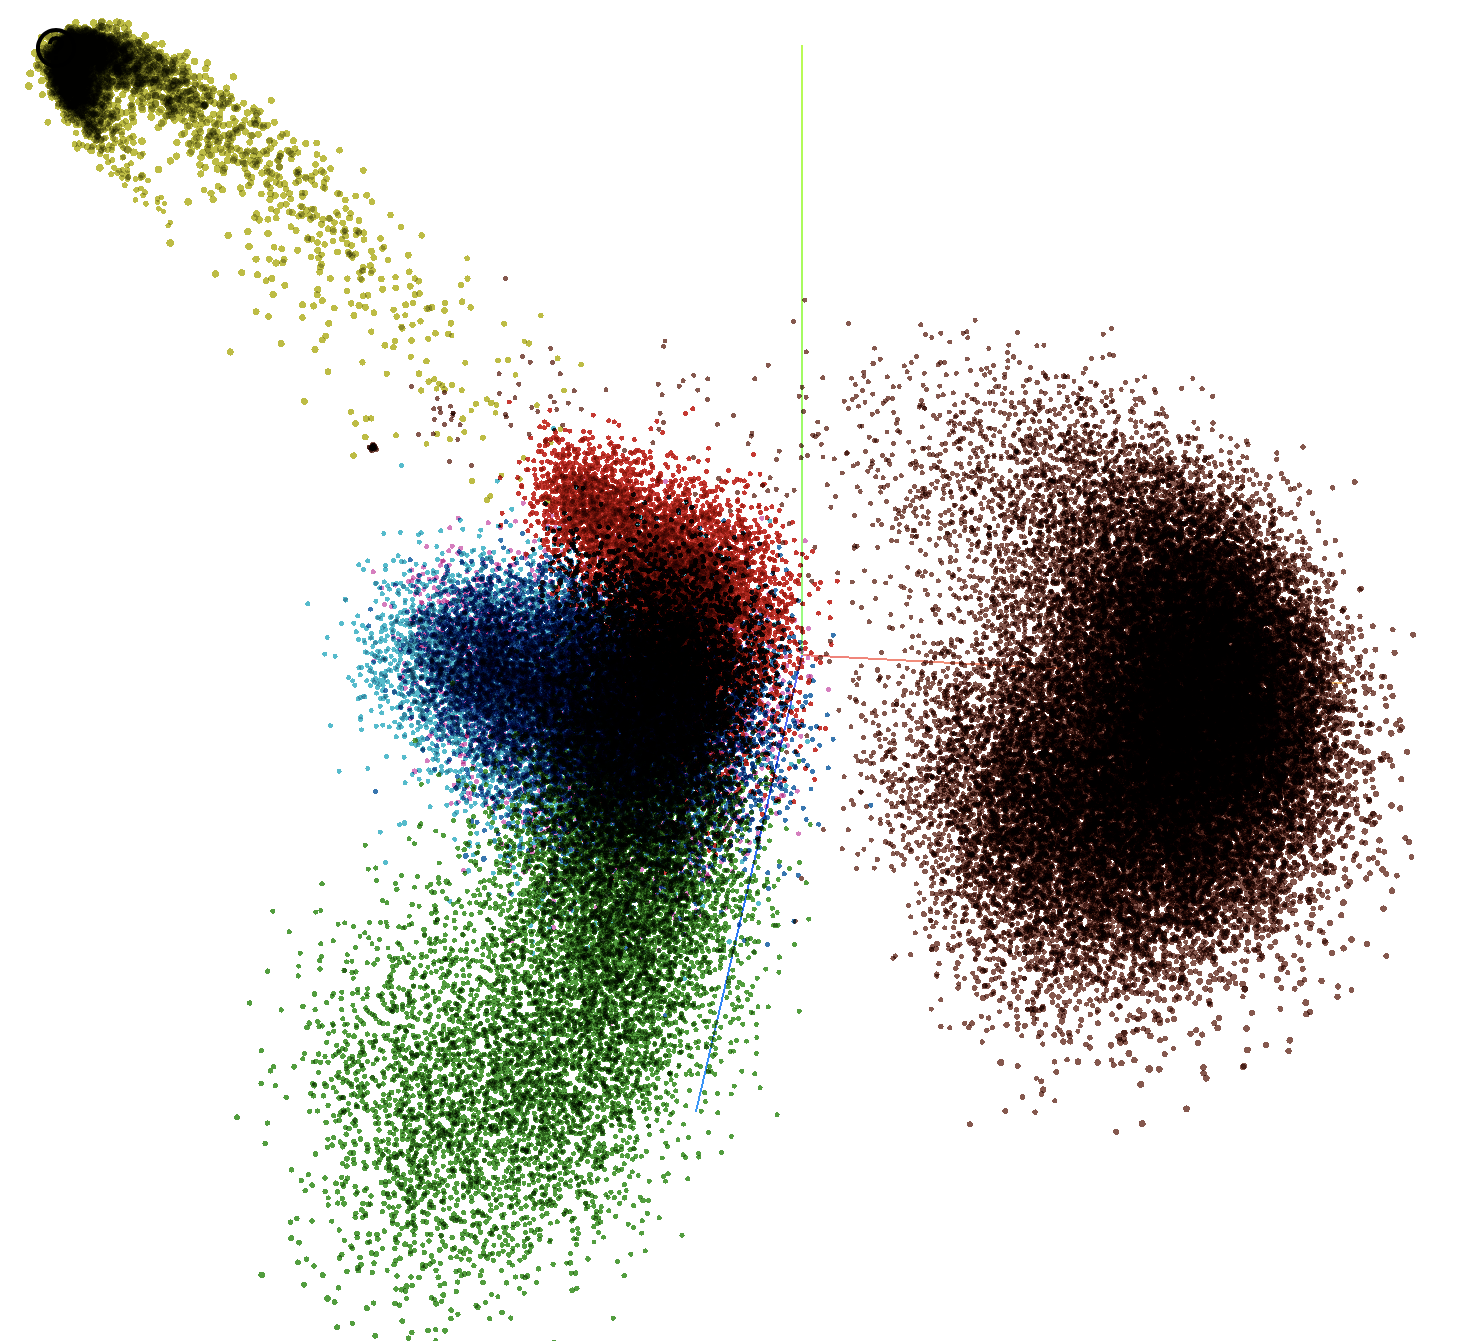
\includegraphics[width=\textwidth]{figures_new/from_old/pca_embedding_projector_2}
  \end{minipage}
    \begin{tablenotes}
      \linespread{1}\footnotesize
      \item[*]\hspace*{-\fontdimen2\font}Total variance described: 34.6\%
      \item[*]\hspace*{-\fontdimen2\font}Tang (dark blue); Song (red); Yuan (pink); Ming (sky blue); Qing (green); 1980s (brown); 2010s (mustard).
    \end{tablenotes}
  \end{threeparttable}
  \caption{Snapshot of PCA Embedding Projector in TensorBoard} \label{fig:tensorboard_PCA}
\end{figure}

\vspace*{\baselineskip}
\begin{figure}[H]
  \centering
  \begin{threeparttable}
  \begin{minipage}[b]{0.45\linewidth}
    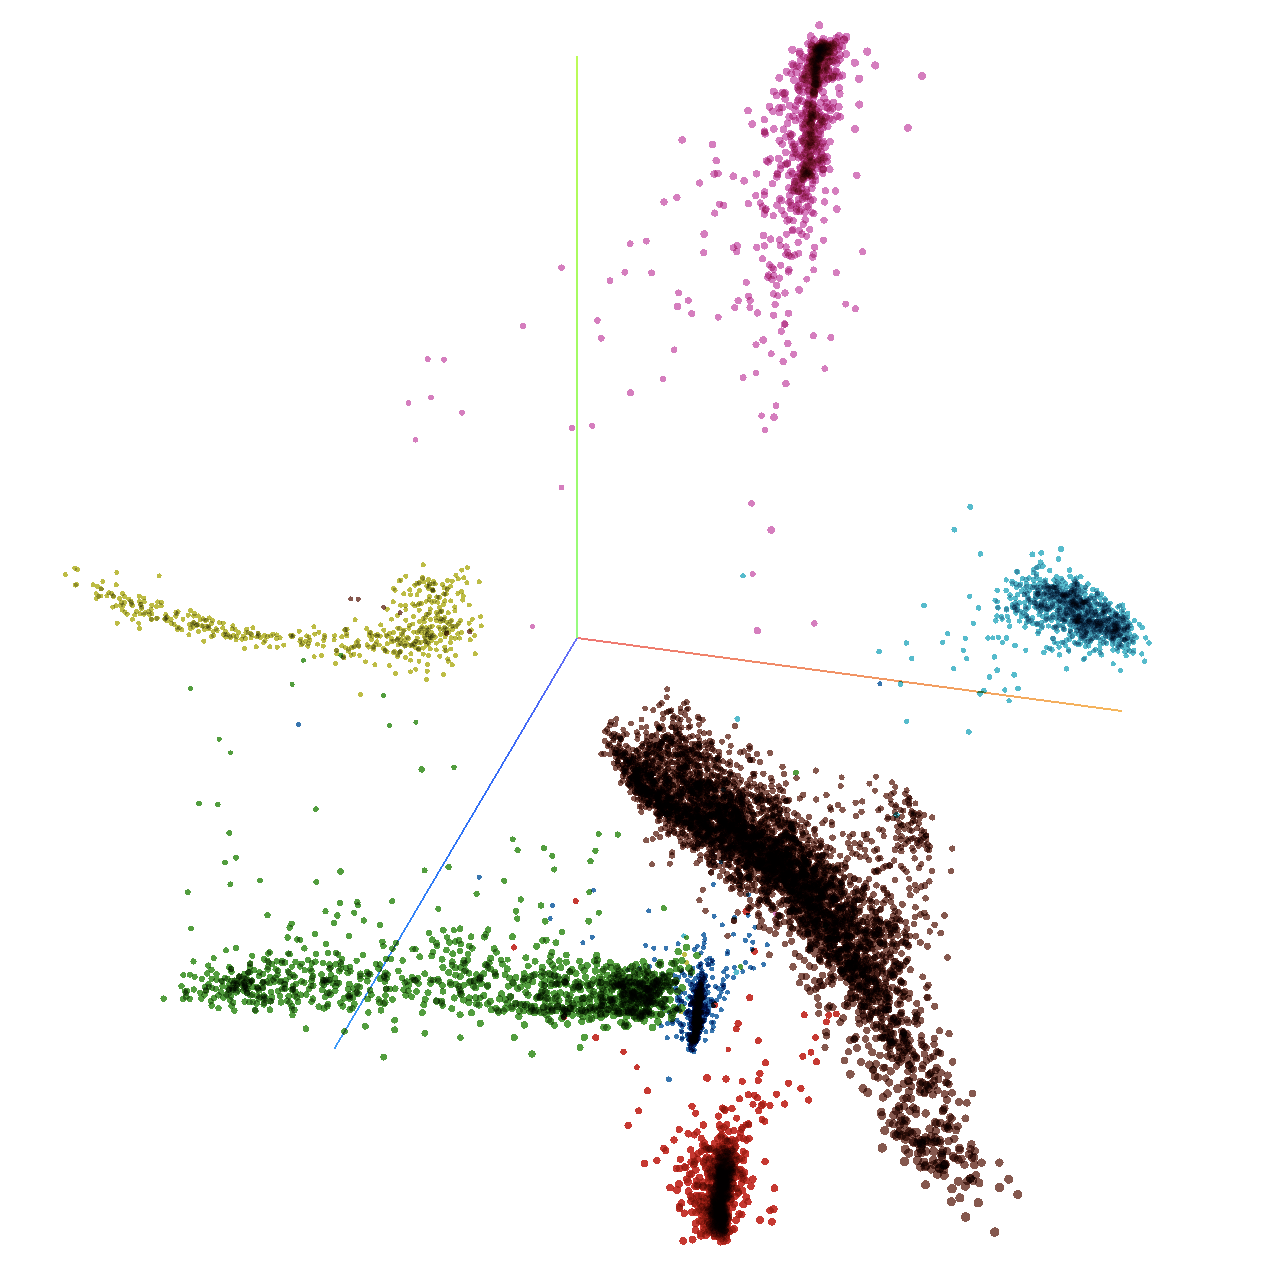
\includegraphics[width=\textwidth]{figures_new/from_old/tsne_embedding_projector_67}
  \end{minipage}
  \quad
  \begin{minipage}[b]{0.45\linewidth}
    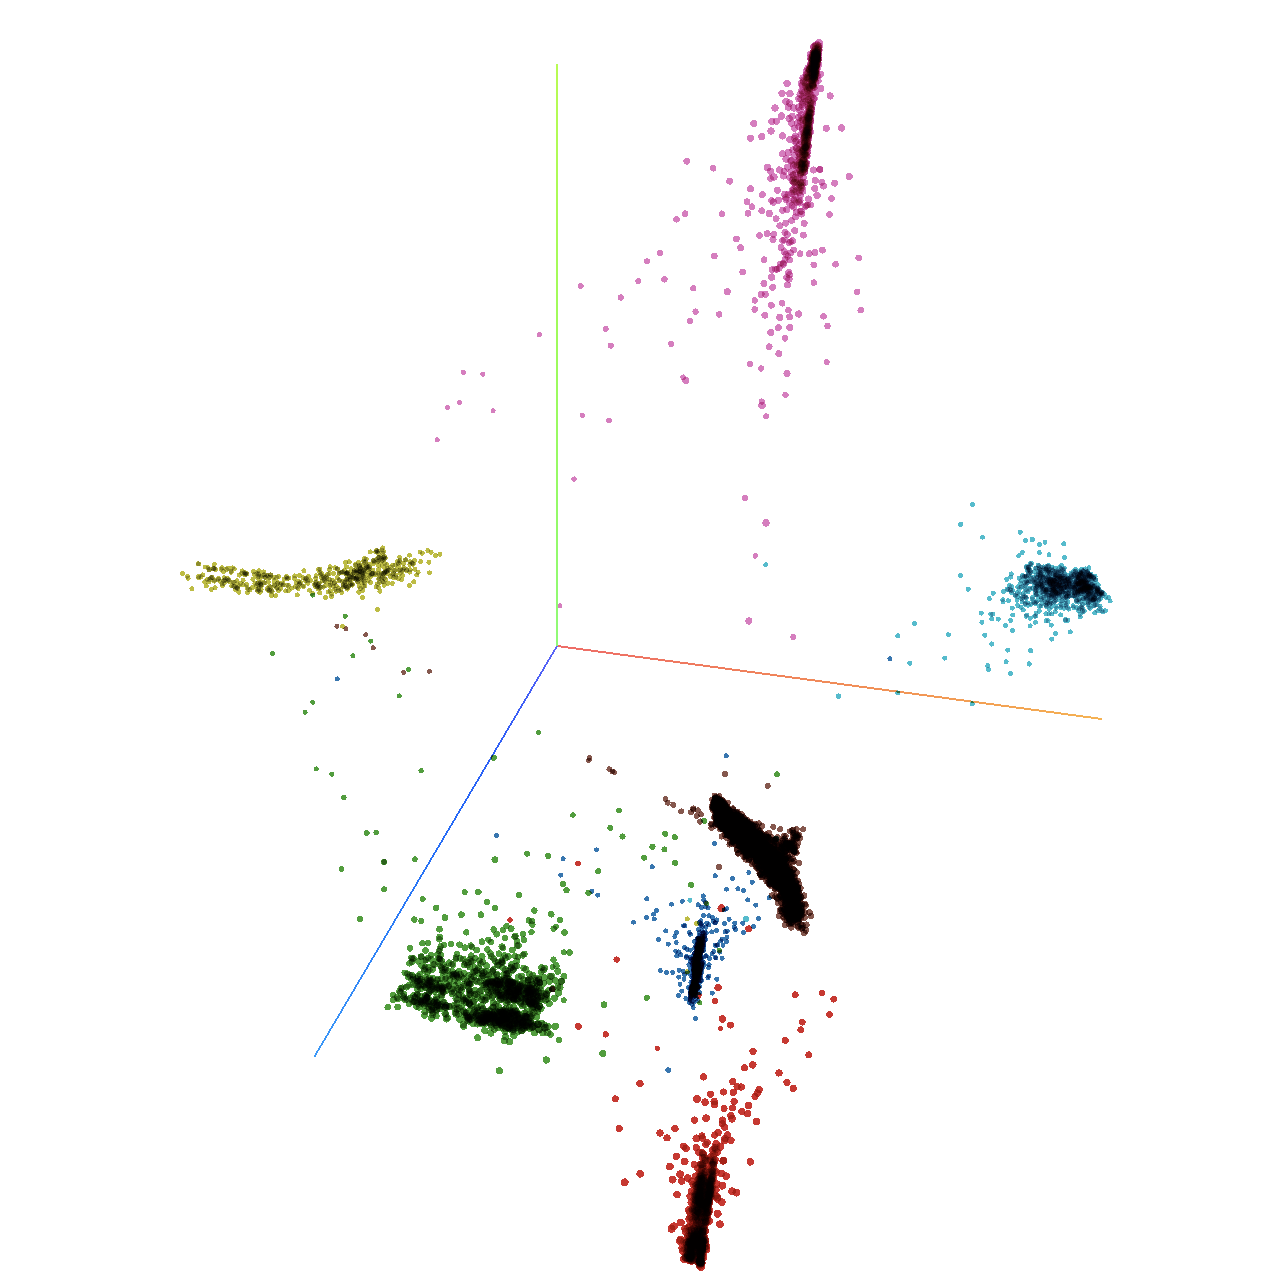
\includegraphics[width=\textwidth]{figures_new/from_old/tsne_embedding_projector_102}
  \end{minipage}
    \begin{tablenotes}
      \linespread{1}\footnotesize
      \item[*]\hspace*{-\fontdimen2\font}Perplexity: 74; learning rate: 10; Iteration: 67 (left panel); 102 (right panel)
      \item[*]\hspace*{-\fontdimen2\font}Tang (dark blue); Song (red); Yuan (pink); Ming (sky blue); Qing (green); 1980s (brown); 2010s (mustard).
    \end{tablenotes}
  \end{threeparttable}
  \caption{Snapshot of t-SNE Embedding Projector in TensorBoard} \label{fig:tensorboard_tSNE}
\end{figure}

\begin{figure}[H]
  \centering
  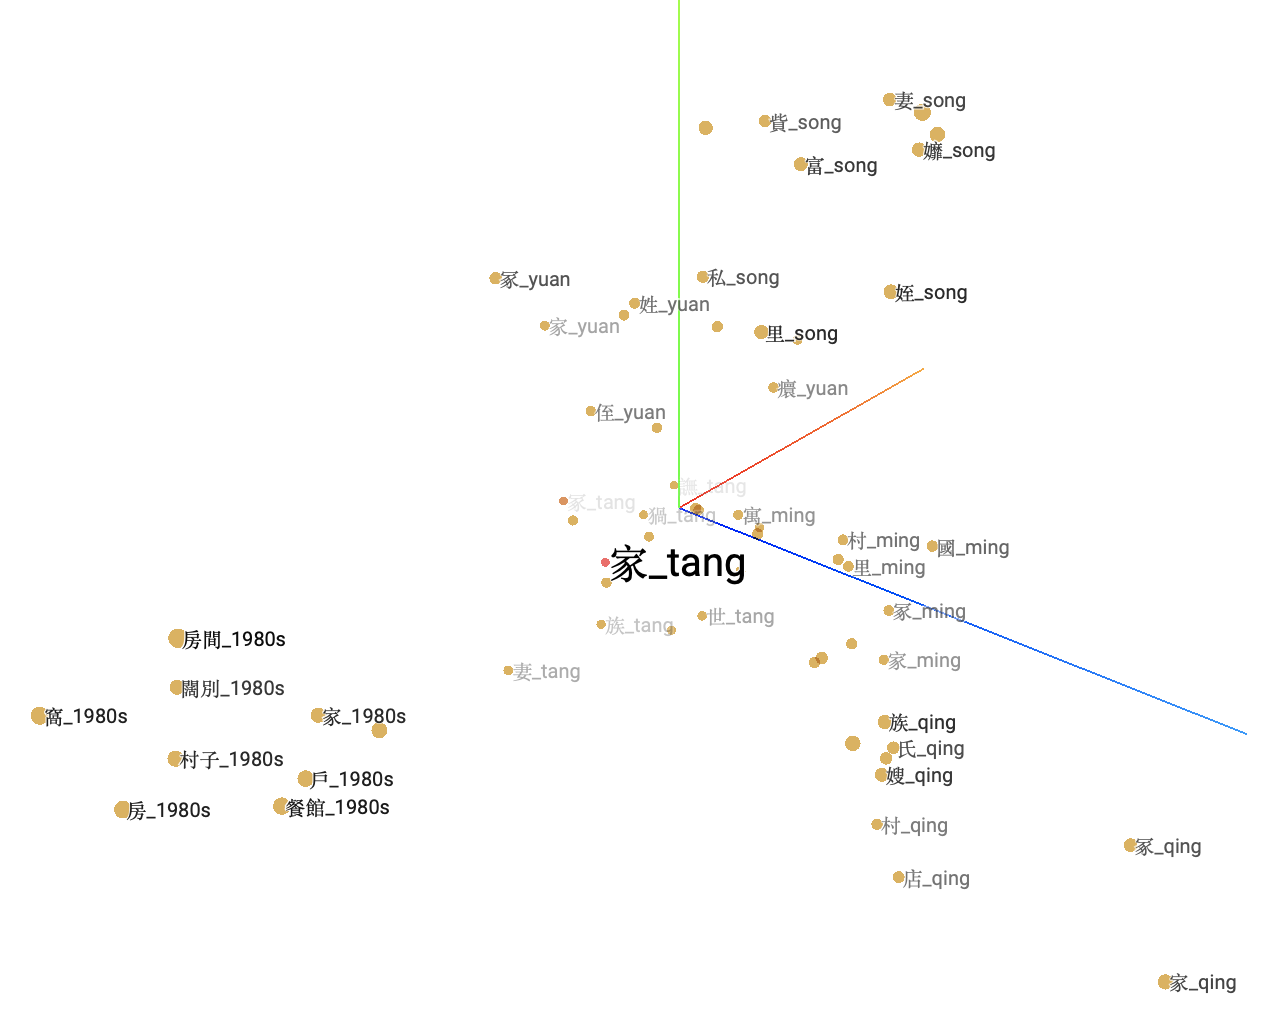
\includegraphics[height=0.475\textheight,width=0.95\textwidth,keepaspectratio]{figures_new/from_old/jia_neighboring_words}
  \caption{Nearest neighbors of \jia projected in three-dimensional space} \label{fig:tensorboard_jia}
\end{figure}

After word-level embeddings from the Tang to Qing dynasty are generated, 20 words with the highest cosine similarity scores of \jia are extracted from each dynasty, as shown in \tref{tab:jia_neighbor_single_char}. Besides the single-character words in pre-modern Chinese, segmented words are also explored for modern Chinese, as shown in \tref{tab:jia_neighbor_segmented}.

In general, it is found that word-level embeddings yield a set of neighboring words with meanings that are close to the definitions listed in the OED and MOE dictionaries. Nonetheless, it is probable that \zh{冢}{zhǒng}{burial mound} tops the list because it could be coded for its resemblance of strokes to \jia, or because the word was also used to refer to family members related to the eldest male offspring, as in \zh{冢嗣}{zhǒngsì}{the eldest male offspring in the family} and \zh{冢婦}{zhǒngfù}{wife of the eldest male offspring}, which is similar to the use of \zh{嫡}{dí}{child of legal wife} \dictcite{zhonginguhanyu}.

\begingroup
\renewcommand{\arraystretch}{0.8}
\begin{table}[H]
  \centering
  \caption{Nearest neighbors of single-character words to \jia} \label{tab:jia_neighbor_single_char}
  \begin{tabularx}{\textwidth}{cp{12.5cm}}
    \toprule
      Dynasty & \multicolumn{1}{c}{Top 20 nearest neighbors} \\
    \midrule
      \csvreader[late after line=\\]%
      {tabs/jia_cat_neighbor_df_premodern.csv}%
      {dynasty=\dynasty, keyword=\keyword}%
      {\dynasty &
      \csvcoliv,  \csvcolv,  \csvcolvi,  \csvcolvii,  \csvcolviii,
      \csvcolix,  \csvcolx,  \csvcolxi,  \csvcolxii,  \csvcolxiii,
      \csvcolxiv,  \csvcolxv,  \csvcolxvi,  \csvcolxvii,  \csvcolxviii,
      \csvcolxix,  \csvcolxx,  \csvcolxxi,  \csvcolxxii,  \csvcolxxiii}
    \bottomrule
  \end{tabularx}
\end{table}
\endgroup

\begingroup
\renewcommand{\arraystretch}{0.8}
\begin{table}[H]
  \centering
  \caption{Nearest neighbors of segmented words to \jia} \label{tab:jia_neighbor_segmented}
  \begin{tabularx}{\textwidth}{cp{12.5cm}}
    \toprule
      Keyword & \multicolumn{1}{c}{Top 20 nearest neighbors} \\
    \midrule
      \csvreader[late after line=\\]%
      {tabs/jia_cat_neighbor_df_modern.csv}%
      {keyword=\keyword}%
      {\keyword &
      \csvcoliv,  \csvcolv,  \csvcolvi,  \csvcolvii,  \csvcolviii,
      \csvcolix,  \csvcolx,  \csvcolxi,  \csvcolxii,  \csvcolxiii,
      \csvcolxiv,  \csvcolxv,  \csvcolxvi,  \csvcolxvii,  \csvcolxviii,
      \csvcolxix,  \csvcolxx,  \csvcolxxi,  \csvcolxxii,  \csvcolxxiii}
    \bottomrule
  \end{tabularx}
\end{table}
\endgroup

The list of nearest neighboring words of \jia can be interpreted from two perspectives. Firstly, considering that the word-level embeddings are built on single characters as words, the nearest neighbors of \jia are able to reflect the concept of home through the three regions delineated by \textcite{sixsmith1986meaning}. Neighboring words such as \zh{父}{fù}{father}, \zh{兄}{xiōng}{elder brother}, \zh{弟}{dì}{younger brother}, \zh{妻}{qī}{wife}, \zh{族}{zú}{family clan}, \zh{世}{shì}{generation;era}, \zh{村}{cūn}{village; country}, \zh{里}{lǐ}{village; neighborhood}, and \zh{鄰}{lín}{village; neighborhood} are evident of the structured social unit of living from the pre-modern time. Interestingly, single-character neighboring words in the 1980s are less likely to capture the meanings of home in the modern time, except for few words that are also in the list of collograms in Section~\ref{results_collocational}.

From another perspective, it is clear that word vectors are able to capture the cultural aspect of \jia in pre-modern Chinese \parencite{hamilton2016cultural}. The core meanings of \jia remain stable from the pre-modern time, indicating a strong association with the family clan and roles of family members. Noticeably, on the list of the most similar words are words related to money, namely \zh{富/冨}{fù}{wealth}, \zh{貧}{pín}{poverty}, \zh{眥}{zì}{to estimate (value)}. In comparison with the collograms in Section~\ref{results_collocational}, \zh{貧}{pín}{poverty} is still consistently seen. Moreover, the pre-collogram \zh{國}{guó}{country;state;feudal land} does not receive a high enough similarity score in the word-level embeddings, but it is the most collocable across multiple time periods.

In view of the distinct difference of the neighboring words in the 1980s, the word-segmented embeddings are also trained for both pre-modern and modern Chinese. As \tref{tab:jia_neighbor_segmented} contains an excerpt of common words to describe the concept of home, the three regions of the personal, social, and physical aspects are successfully captured, as in \zh{村子}{cūnzi}{village}, \zh{家小}{jiāxiǎo}{wife and children}, \zh{養老院}{yǎnglǎoyuàn}{nursing home} for the keyword \jia\rspace. It is believed that other keywords are also capable of gaining an insight into the cultural aspect of home in modern Chinese. Nonetheless, although words such as \zh{族}{zú}{family clan} are not ranked as top nearest neighbors, it does not entail that the word becomes less semantically related to the concept of home in modern Chinese, but suggests that other keywords are more likely to answer this question. For instance, the neighboring words of the keyword \zh{家族}{jiāzú}{family clan} are indicative of the shift of family clans as units of living to smaller household sizes and more equal status of each family member, as in \zh{主婦}{zhǔfù}{housewife}, \zh{職業婦女}{zhíyè fùnǚ}{career woman}, \zh{小家庭}{xiǎojiātíng}{nuclear family}.

Besides, terms of commercial properties are spurring in the list of the most similar words to \jia in the 1980s, and the neighboring words with the highest similarity score is \zh{店}{diàn}{store}. It is speculated that commercialization is accountable for this new trend, and it is also possible that \jia starts to be used as a classifier, as in \zh{一家麵包店}{yì jiā miànbāodiàn}{a bakery}. Yet, this trend of commercialization and the use of classifier is not in parallel with the collograms.

Following \textcite{antoniak2018evaluating}, the semantic change of the keyword \jia is further analyzed in the \sctext{bootstrap} settings in order to address the issue of uncertainty in the \sctext{fixed} settings. Particularly, the cosine similarity scores and ranks of nearest neighbors are used as the metrics to filter out those that might be less stably seen in the results, as shown in \fref{fig:bootstrap_mean_sd} and \fref{fig:bootstrap_rank}.

In the 1980s, the single-character neighboring words are much more unstable than the segmented counterparts, as indicated by the low similarity scores and unevenly dispersed ranks. Furthermore, specific terms of commercial properties tend to exhibit high variability in the 1980s, whereas words like \zh{村子}{cūnzi}{village} and \zh{房間}{fángjiān}{room} are still closely related to the keyword \jia\rspace. Regarding \zh{店}{diàn}{store}, which has the highest similarity score to \jia\rspace , has an even higher mean for the scores in the bootstrap samples, along with a narrow distribution of ranks. In pre-modern Chinese, the cosine similarity scores are more consistent between the two settings, and rare words stand out with a much higher variability. Therefore, it can be concluded that treating single characters as words is more revealing than segmenting pre-modern texts to extract semantically related words.

\newpage
\begin{figure}[H]
  \centering
  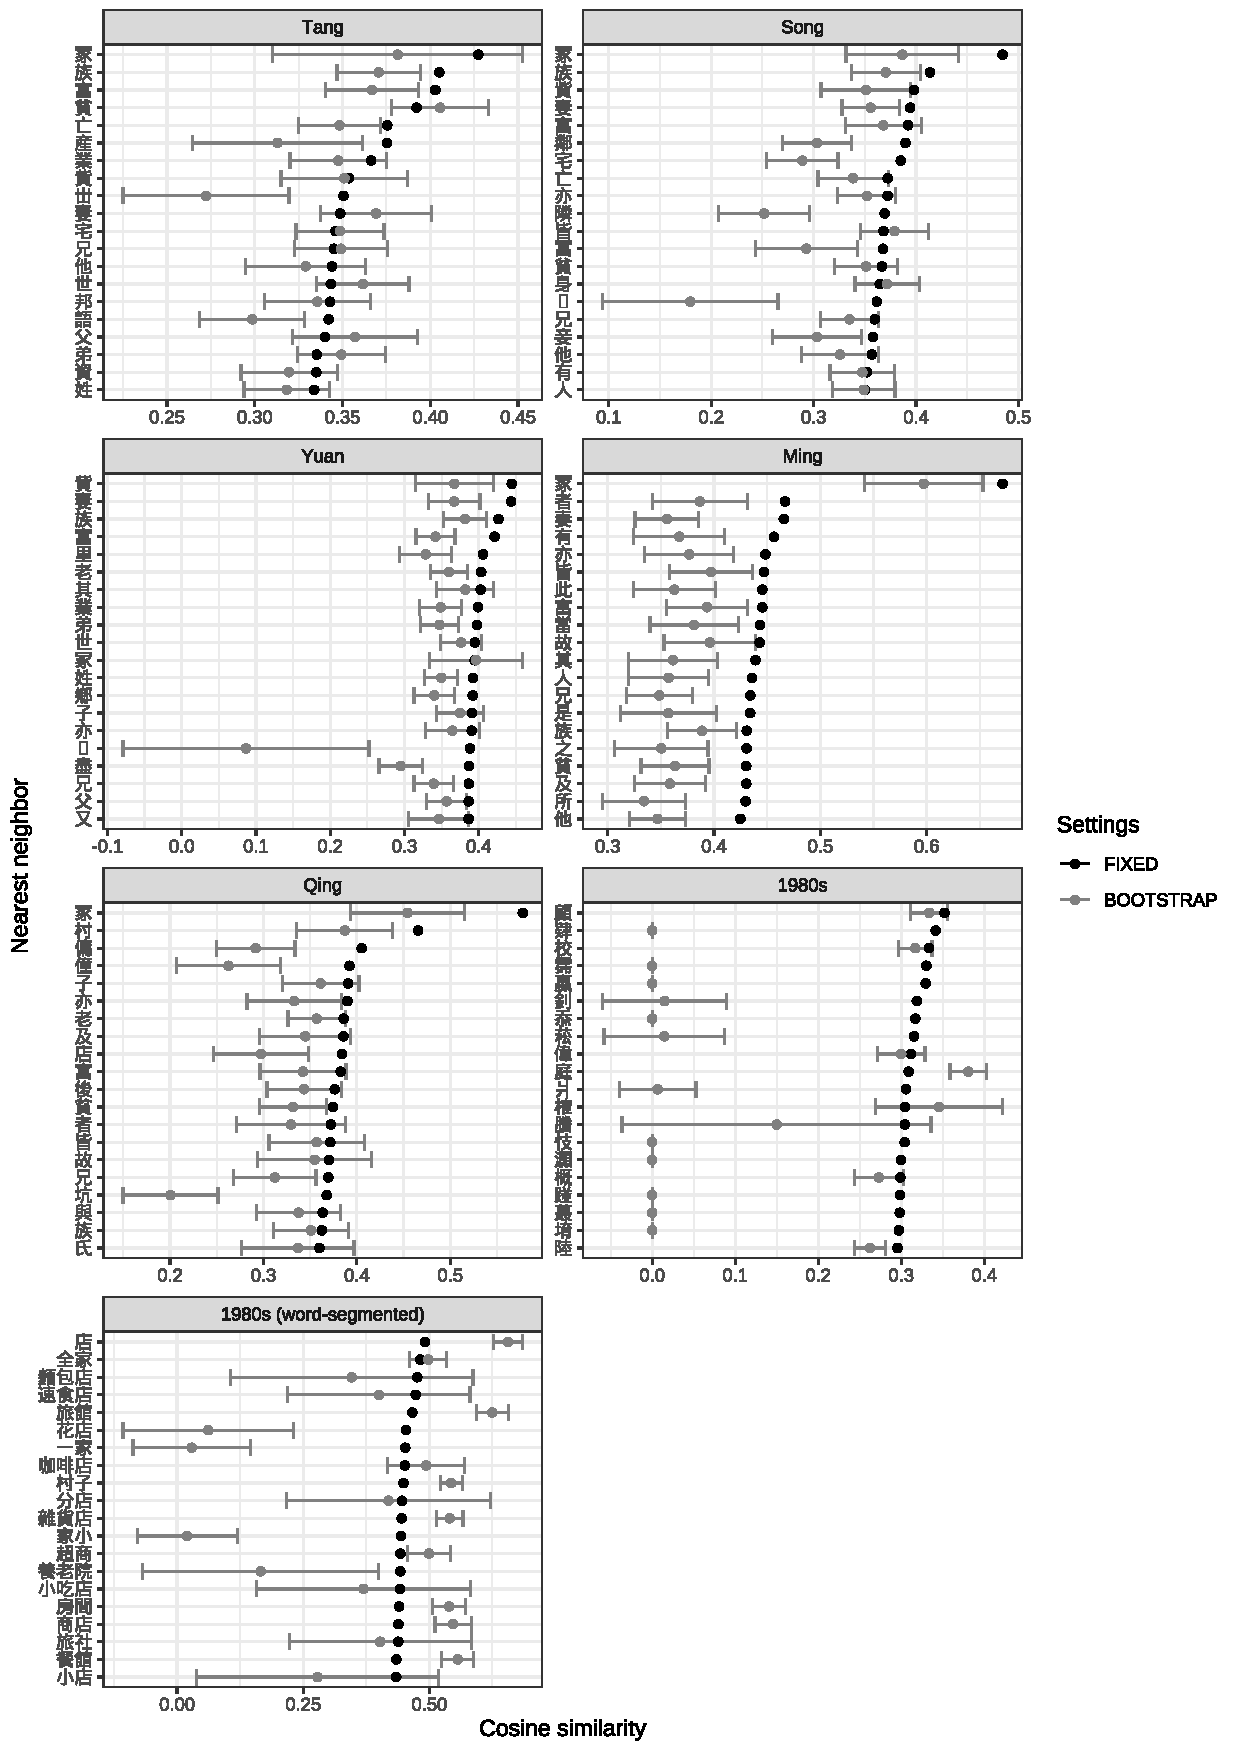
\includegraphics[height=0.85\textheight,keepaspectratio]{figures_new/bootstrap_for_stability/neighbor_mean_and_sd_grey.pdf}
  \caption{Nearest neighbors of \jia with means and standard deviations of cosine similarities derived from word-level embeddings in the \sctext{fixed} and \sctext{bootstrap} settings. The 20 nearest neighbors are selected from the \sctext{fixed} settings, and word-segmented embeddings are included for the time period of 1980s.} \label{fig:bootstrap_mean_sd}
\end{figure}

\newpage
\begin{figure}[H]
  \centering
  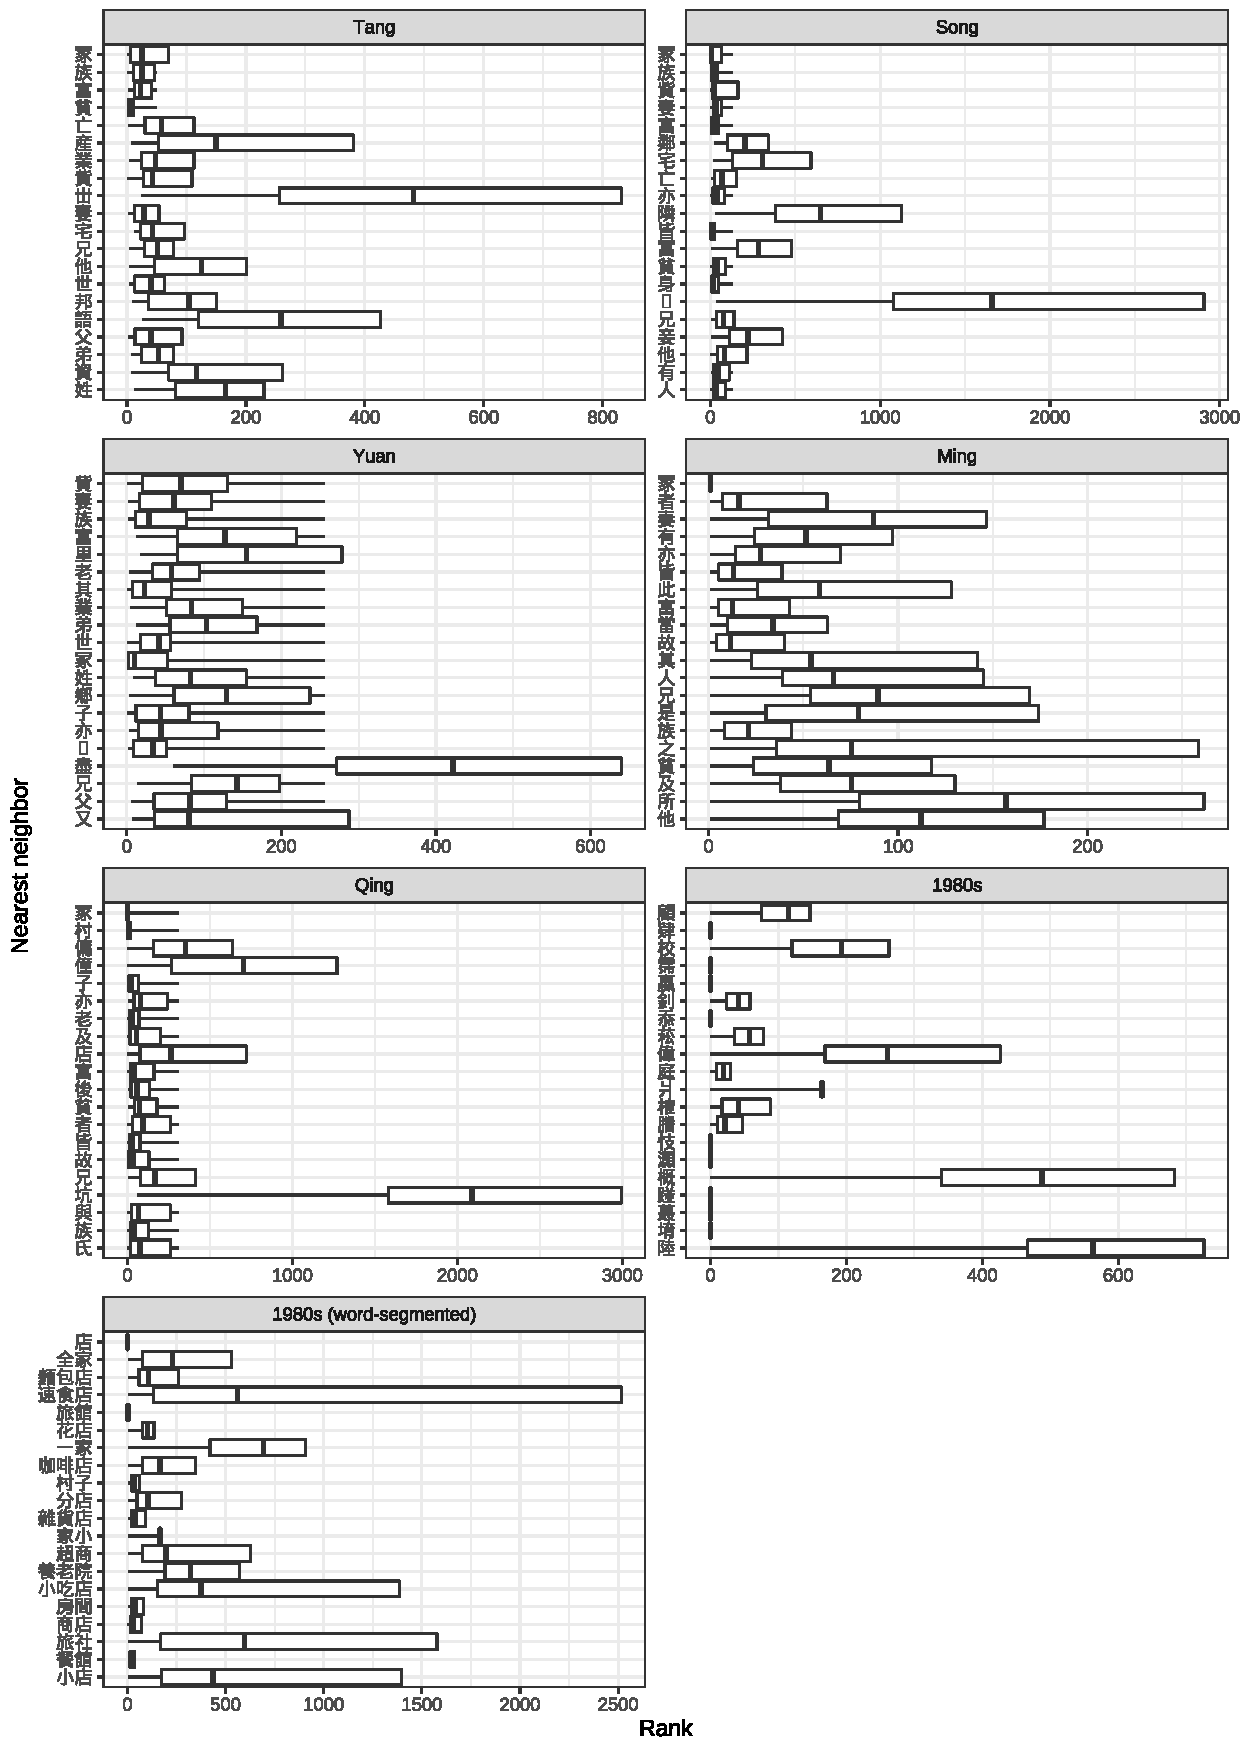
\includegraphics[height=0.85\textheight,keepaspectratio]{figures_new/bootstrap_for_stability/neighbor_rank_change.pdf}
  \caption{Nearest neighbors of \jia with changes in rank derived from word-level embeddings in the \sctext{bootstrap} settings. The 20 nearest neighbors are selected from the \sctext{fixed} settings, and word-segmented embeddings are included for the time period of 1980s.} \label{fig:bootstrap_rank}.
\end{figure}

\section{Sense-level Embeddings}
Although the application of word-level embeddings grows increasingly popular to , it has been criticized for representing words with multiple meanings as one single vector, which is referred to as ``meaning conflation deficiency'' \parencite{camacho2018survey} To allow the algorithms to know different senses of the same word form, two main methods for sense embeddings are proposed. [21, 22] One is unsupervised as senses are ``induced'' from the training corpora; the other is knowledge-based, meaning external sense inventories, such as WordNet, are required to fine-tune the word vector models.

\begin{figure}[H]
  \centering
  \includegraphics[width=0.95\textwidth]{figures_new/diachronic_sense_modeling/家_zh.png}
  \caption{Diachronic interactions of senses of \jia in Chinese WordNet (CWN)}
  \label{fig:jia_polynomial}
\end{figure}

The extraction of contextualized embeddings allows for a sketch of usage distribution displayed by proportion and interactions of different senses, as shown in \fref{fig:jia_polynomial}. From \fref{fig:jia_polynomial}, it is shown that senses do compete and cooperate semantically. In present-day Chinese, sense 1 (family), sense 3 (house), and sense 7 (-ist) are shown to be three of the most prominent senses, yet sense 1 does not evolve in identical direction with sense 3 and 7 in Song and Ming. Instead, its rise of sense 1 has indicated that single-character words like \jia can be read as `family', and combined with sense 3, they account for over 60 percent of the usage proportion, while sense 7 is only half of it. Interestingly, both sense 7 and 8 carry the meaning of describing someone's profession, but the contextualized embeddings distinguish the two readings in terms of the percentage. Qualitatively, these are influenced by different schools of thought. Furthermore, it is comparatively rare for \jia to serve as adjective `domestic', or sense 10 as categorical name.

Firstly, Sense 1 and Sense 3 have the highest proportions in the 1980s. This prevalence follows a rapid growth in the use of the two senses. Nonetheless, the evolvement of Sense 3 is more non-monotonous than that of Sense 1 although the two senses start to share a similar upward trend from the Qing dynasty. It is also interesting that Sense 2 takes up around 2\% to 5\% (5.3\%, 2.4\%, 5.1\%, 2.9\%, 2.4\% from the Tang to Qing dynasty respectively) of the overall proportion in pre-modern Chinese. Semantically, both Sense 2 and 3 can be used to refer to \jia as a physical entity, whereas Sense 1 describes \jia as a social unit, as in \exref{ex:family} to \exref{ex:house_1980s}. 

The fluctuation of Sense 3 might be a result of the distinguishment of this sense from a similar one, Sense 2, as exemplified in \exref{ex:settle_down}.  In contrast, the upward curve of Sense 1 is sharpe, which embodies the expression of \jia as a social unit. Yet, it is also found that the results of these three senses include sentences with bi-grams of \jia that do not have a corresponding pre-determined sense, e.g., \zh{國[家]}{guójiā}{country; state}, \zh{奴[家]}{nújiā}{your servant (humble self-reference by young female)}, as in \exref{ex:country} and \exref{ex:your_servant}. When a belonging sense is unavailable, it is challenging to disambiguiate the meanings given the token representations. It is especially attributable if an example sentence contains wider context information that obscures the results.

\begin{exe}
  \ex{
    \begin{xlist}
      \ex{
        \sent{吾[家\_1]先人}%
        {My ancestors}%
        {Yuan}{至正直記}
        \label{ex:family}
      }
      \ex{
        \sent{奴[家\_1*]把布接長}%
        {I, your servant, hold the clothes together to make it a long one}%
        {Ming}{醒世恆言}
        \label{ex:your_servant}
      }
    \end{xlist}
  }
  \ex{
    \begin{xlist}
      \ex{
        \sent{始[家\_2?]咸陽焉}%
        {(He) originally settled down in Xianyang.}%
        {Song}{廣卓異記}
        \label{ex:settle_down}
      }
      \ex{
        \sent{余曾至其[家\_3]食}%
        {I once went to his house and had a meal there.}%
        {Tang}{古清涼傳}
        \label{ex:house_Tang}
      }
      \ex{
        \sent{在住[家\_3]附近經常可以聽到嘰嘰嘰的蟲鳴聲}%
        {You will often hear the chirping insects near your house.}%
        {1980s}{\gls{asbc}}
        \label{ex:house_1980s}
      }
      \ex{
        \sent{豈可於國[家\_3*]艱危之時而自圖安閒}%
        {How could I seek a carefree life for myself while the country is at stake.}%
        {Song}{建炎進退志}
        \label{ex:country}
      }
    \end{xlist}
  }
\end{exe}

In modern Chinese, Sense 7, 8, 9 are profession-related senses, as in \zh{美聲[家]}{měishēngjiā}{bel canto singer}, \zh{樵[家]和獵[家]}{qiáojiā hàn lièjiā}{woodman and hunter}, and \zh{儒墨兩[家]}{rúmòliǎngjiā}{the Confucian and Mohist schools}. Despite being semantically similar, only Sense 8 and 9 evolve cooperatively, whereas Sense 7 is seen to compete against these two senses. A steep downward curve is seen for both Sense 8 and Sense 9 in the Qing dynasty (from 24.8\% and 15.5\% in the Qing dynasty to 3.7\% and 2.5\% in the 1980s), while Sense 7 surges in use during the same time period, and continues to be more and more prominent in the 1980s (from 2.2\% in the Qing dynasty to 17.6\% in the 1980s). Professions like \zh{醫[家]}{yījiā}{doctor}, \zh{史[家]}{shǐjiā}{historian}, and \zh{詩[家]}{shījiā}{poet}, as in \exref{ex:doctor} through \exref{ex:poet}, are mapped to Sense 7 in pre-modern Chinese, and a wide variety of occupations are included for the same sense in modern Chinese, which contributes to the rise and prominence of Sense 7 in the 1980s.

\begin{exe}
  \ex{
    \begin{xlist}
      \ex{
        \sent{醫[家\_7]治痘斑之法}%
        {Doctors' acne spot treatments.}%
        {Qing}{痘疹心法要訣}
        \label{ex:doctor}
      }
      \ex{
        \sent{然史[家\_7]多是文詠之士}%
        {Oftentimes, historians are rather thought of as writers of poetry and prose.}%
        {Song}{孔氏雜說}
      }
      \ex{
        \sent{此所謂詩[家\_7]之中道也}%
        {This is the so-called teaching of poets.}%
        {Tang}{文鏡秘府論}
        \label{ex:poet}
      }
      \ex{
        \sent{我是組織生態學[家\_7]}%
        {I'm an organizational ecologist.}%
        {1980s}{\gls{asbc}}
      }
      \ex{
        \sent{英文的同時有道教信徒和道士和道[家\_7*]的意思}%
        {In English, it can refer to Taoist followers, Taoist priests, and Taoism.}%
        {1980s}{\gls{asbc}}
      }
    \end{xlist}
  }
  \ex{
    \begin{xlist}
      \ex{
        \sent{莫孤負田[家\_8]瓦盆}%
        {Do not disobey the family precepts of a farmer}%
        {Yuan}{類聚名賢樂府群玉}
        \label{ex:farmer}
      }
      \ex{
        \sent{窮人[家\_8*]的男子}%
        {A man from a poor family.}%
        {1980s}{\gls{asbc}}
      }
    \end{xlist}
  }
  \ex{
    \begin{xlist}
      \ex{
        \sent{自漢至明修輯者七十餘[家\_9]}%
        {More than 70 names edited and compiled the works from the Han to Ming dynasty.}%
        {Qing}{乾元秘旨}
      }
      \ex{
        \sent{漁翁不謂其出[家\_9*]人不宜食魚}%
        {The fisherman does not think he, as a monk, should abstain from having fish.}%
        {Ming}{第十一尊杯渡羅漢}
        \label{ex:monk}
      }
    \end{xlist}
  }

\end{exe}

On top of that, regarding the proportion of usage, Sense 10, 11, and 12 consistently rank the lowest in pre-modern Chinese, but a sudden increase is witnessed for Sense 11 and 12 in the 1980s. Among all the 18 senses of \jia\rspace , Sense 12 is the only one acting as a classifier, or Nf in the \gls{asbc} tagset.

\begin{exe}
  \ex{
    \sent{除了選擇一[家\_10]好的\ldots}%
    {Apart from choosing one good brand\ldots}%
    {1980s}{\gls{asbc}}
  }
  \ex{
    \begin{xlist}
      \ex{
        \sent{但臺灣建築業者號稱上萬[家\_11]}%
        {Yet it is claimed that there are up to ten thousands of construction companies in Taiwan.}%
        {1980s}{\gls{asbc}}
      }
      \ex{
        \sent{頭一[家\_11]做生意就勿高興出來}%
        {The first time he opened up business, he was unhappy.}%
        {Qing}{海上花列傳}
      }
  \end{xlist}
  }
  \ex{
    \begin{xlist}
      \ex{
        \sent{\ldots 列有四百五十[家\_12]值得信賴的商店}%
        {\ldots lists out 450 brands that are trustworthy.}%
        {1980s}{\gls{asbc}}
      }
      \ex{
        \sent{是省城第一[家\_12?]好主戶}%
        {They are the best settled household around capital.}%
        {Qing}{歧路燈}
      }
    \end{xlist}
  } 
\end{exe}

Sense-level embeddings are capable of capturing fine-grained senses and their evolution, yet the contextual information provided from pre-modern Chinese sentences might not be sufficient enough to accurately map the token representations to their belonging senses from the pre-trained language model.

% \begin{exe}
%   \ex
% (Sense 7)\\
% 又以堪輿\CJKfakebold{家}所謂龍脈也 \parencite{sturgeon2019ctext}\\
% yòu\_\_yǐ\_\_kānyújiā\_\_suǒwèi\_\_lóngmài\_\_yě\\
% additionally\_\_P\_\_geomantician\_\_so-called\_\_dragon's-vein\_\_PAR\\
% \textit{what[=the terrain] a geomantician would call a dragon's vein}
% \end{exe}

The polysemy of a lexical item is addressed by constructing multiple contextualized token embeddings. Shades of meanings are reflected in the diversity of contextual use.

The results indicate that \jia enjoy far global distance but low local distance, and suddenly rises during 1980s.

% 1. average silhouette width \parencite{levshina2015linguistics}
% Rectangles with the optimal number of clusters, according to the average silhouette widths

% 2. snake plot

% 3. effect size measure

\section{Discussion}
Following \textcite{hamilton2016law}, in which the evaluation is based on examples from previous works on semantic change and words with the ``obsolete'' tag in the Oxford English Dictionary (OED), dictionary entries are consulted to look for ``舊時'' and ``古代'' for attested examples to evaluate the trained diachronic word embeddings.

For example, \zh{齒}{chǐ}{tooth} used to carry the meaning `age (年齡)' and `being of equal rank (並列)' because age determination is made by numbering horses' teeth, which emerges one each year, as in `子之齒長矣,不能事人 (You are long in the tooth)' and `不敢與諸任齒 (I would not dare to take rank equivalent to yours)'; another example is \zh{卑鄙}{bēi-bǐ}{despicable}, which is more neural in connotation in the past \parencite[前言]{wang1997gujinyiyi}. Dictionaries include \textcite{wang1997gujinyiyi,liu1992gujinyi}, which lists word entries with meanings that are distinctive between modern and pre-modern times. Detailed information relevant to semantic change is the number of disyllabic word entries, whether the word convey connotations with varying sentiment polarities, and whether certain senses fall into disuse nowadays, which is valuable resources for the comparison with the results of computational methods. However, the division of time periods, or the granularity, examined in previous studies, especially those on laws of semantic change, is restricted to the nineteenth century onward. Additionally, to trace semantic change of a language, it is necessary to account for the development of words at the interface of morphology and semantics. Therefore, we aim to analyze both pre-modern and modern Chinese texts, which would be the first attempt to apply both computational and statistical models to explore the interplay between disyllabic development of words and semantic change in Chinese.

% topic modeling
\begin{figure}[H]
  \centering
  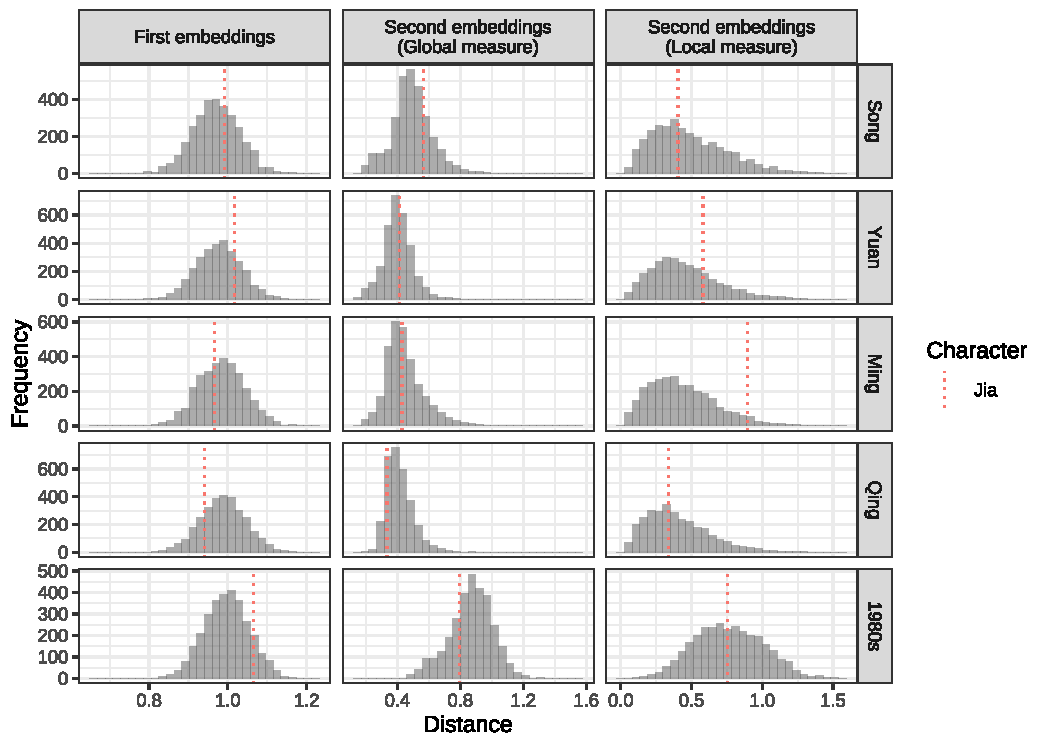
\includegraphics[width=0.75\textwidth,keepaspectratio]{figures_new/measures/dist_hist_w5.pdf}
  \caption{Distribution of degree of semantic change measured globally and locally}
\end{figure}

The meanings are based on 漢語大字典, 漢語大詞典, 辭源, 辭海 as well as 現代漢語詞典 and 新華詞典 (both published by 商務印書館).

frequency data is derived from 在线古代汉语语料库字频数据\footnote{\url{http://corpus.zhonghuayuwen.org/resources.aspx}} and 近代漢語語料庫詞頻統計\footnote{\url{https://elearning.ling.sinica.edu.tw/jindai.html}}, which are the metadata from the 70-million-word Ancient Chinese Corpus (在线古代汉语语料库) by the Ministry of Education, China and Academia Sinica Tagged Corpus of Early Mandarin Chinese (近代漢語語料庫) by Academia Sinica, Taiwan.

The case study of \jia is based on the assumption that the time-sliced corpus might reflect the similar and different descriptions in language use. While words in \tref{use_case} fall into the categories of technological innovations and ideologies, this study chooses \jia because of its linguistic and cultural characteristics. In pre-modern Chinese, \jia is associated with words that denote physical objects like house.

Because the corpus contains multiple versions of a document, some orthographically-similar characters rank top in terms of cosine similarity scores. However, if compared with the results from \sctext{bootstrap} samples, the scores are widest. In addition, the ranks vary widely in different iterations, and are a reliable indicator of neighbor analysis. For example, \zh{貧}{pín}{poor;impoverished} appear 43 times out of the 50 iterations as the top 20 closest neighbors, followed by \zh{窶}{jù}{poor;impoverished} also appear 26 times. Other closest neighbors include 族, 世, 妻, 冢, 富, \zh{寠}{jù}{poor;impoverished}, 孀, 糿, 父 (all more than 15 times.)

As for the word 宅, the closest neighbors include 田(48), 廨(47), 居(39), 園(36), 墅(36), 家(35), and 廛(14), filtering out 冢(1). Compared with \sctext{fixed} embeddings, the closest neighbors for the Tang dynasty include 廨, 田, 宇, 邸, 園, 營, 室, 塋, 寺, 住, 妝, 寓. Therefore, if neighbor analysis can be compared from two directions, it is likely to mitigate the issue arising from OCR errors?

The semantic history of linguistic units or expressions are far more unpredictable than data that contain seasonality. Regarding the closet neighbors for \jia , the results differ in a distinctive way, with a low percentage of overlaps between the \sctext{fixed} embeddings and the \sctext{bootstrap} ones. In addition, before the diachronic character-based embeddings are constructed, a decision needs to be made on whether the different versions of a workset of texts are to be included or excluded. Considering the fact that the documents are converted from scanned copies to the digital texts in UTF-8 encoding using the OCR technique, the \sctext{fixed} embeddings reinforce the parts that are consistently recognizable and transformed into similar strings of characters. In other words, the inclusion of all versions in a workset of documents prevents misrecognized characters from taking up a significant portion of the word occurrence behavior. On the other hand, the word co-occurrence profile remains susceptible to orthographically highly similar characters, e.g., 家 and 冢, 人 and 入, and 怡 and 恰, and place the mistaken form as the close neighbors, oftentimes the closest neighbor.

\newpage
\begin{figure}[H]
    \centering
    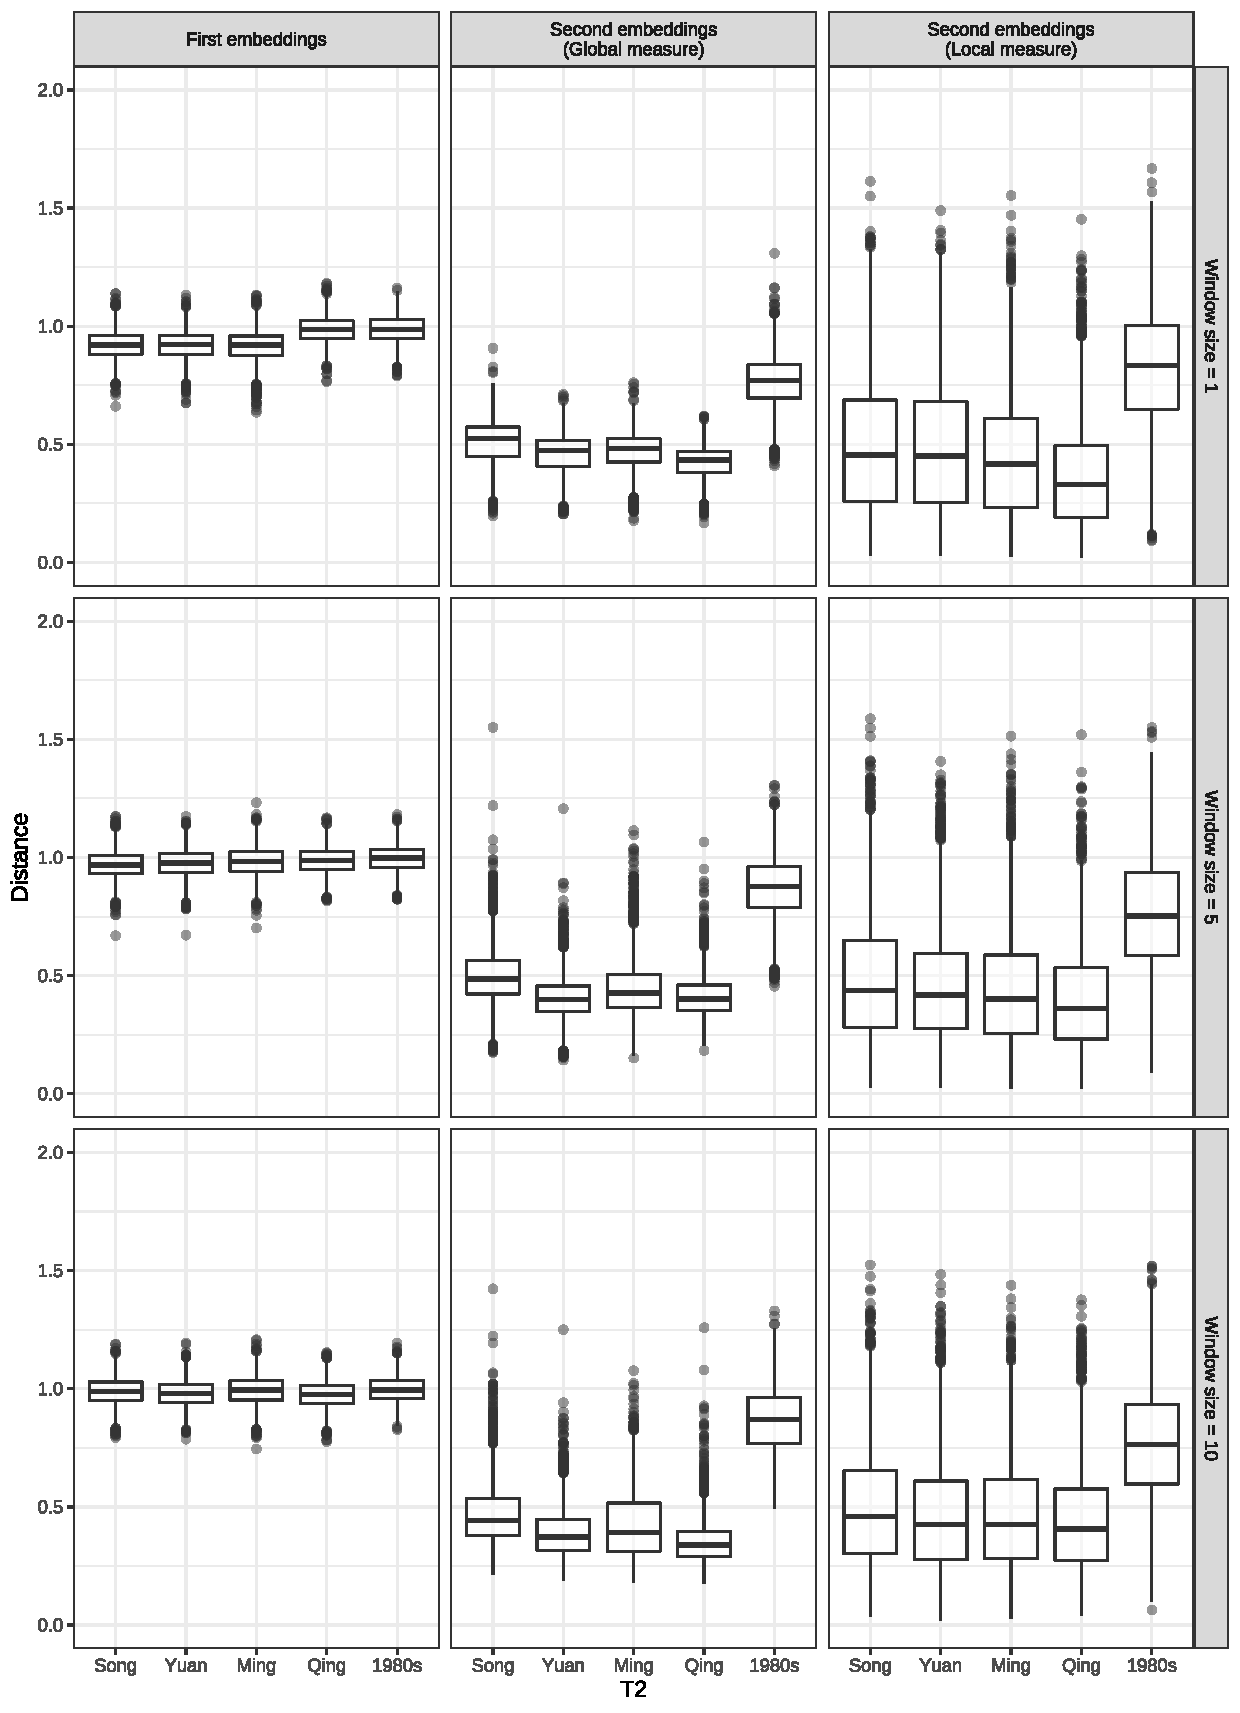
\includegraphics[width=0.95\textwidth,height=0.95\textheight,keepaspectratio]{figures_new/measures/dist_boxplot.pdf}
    \caption{Distribution of degree of semantic change measured globally and locally}
\end{figure}

\newpage
\begin{figure}[H]
  \begin{subfigure}{0.3\textwidth}
    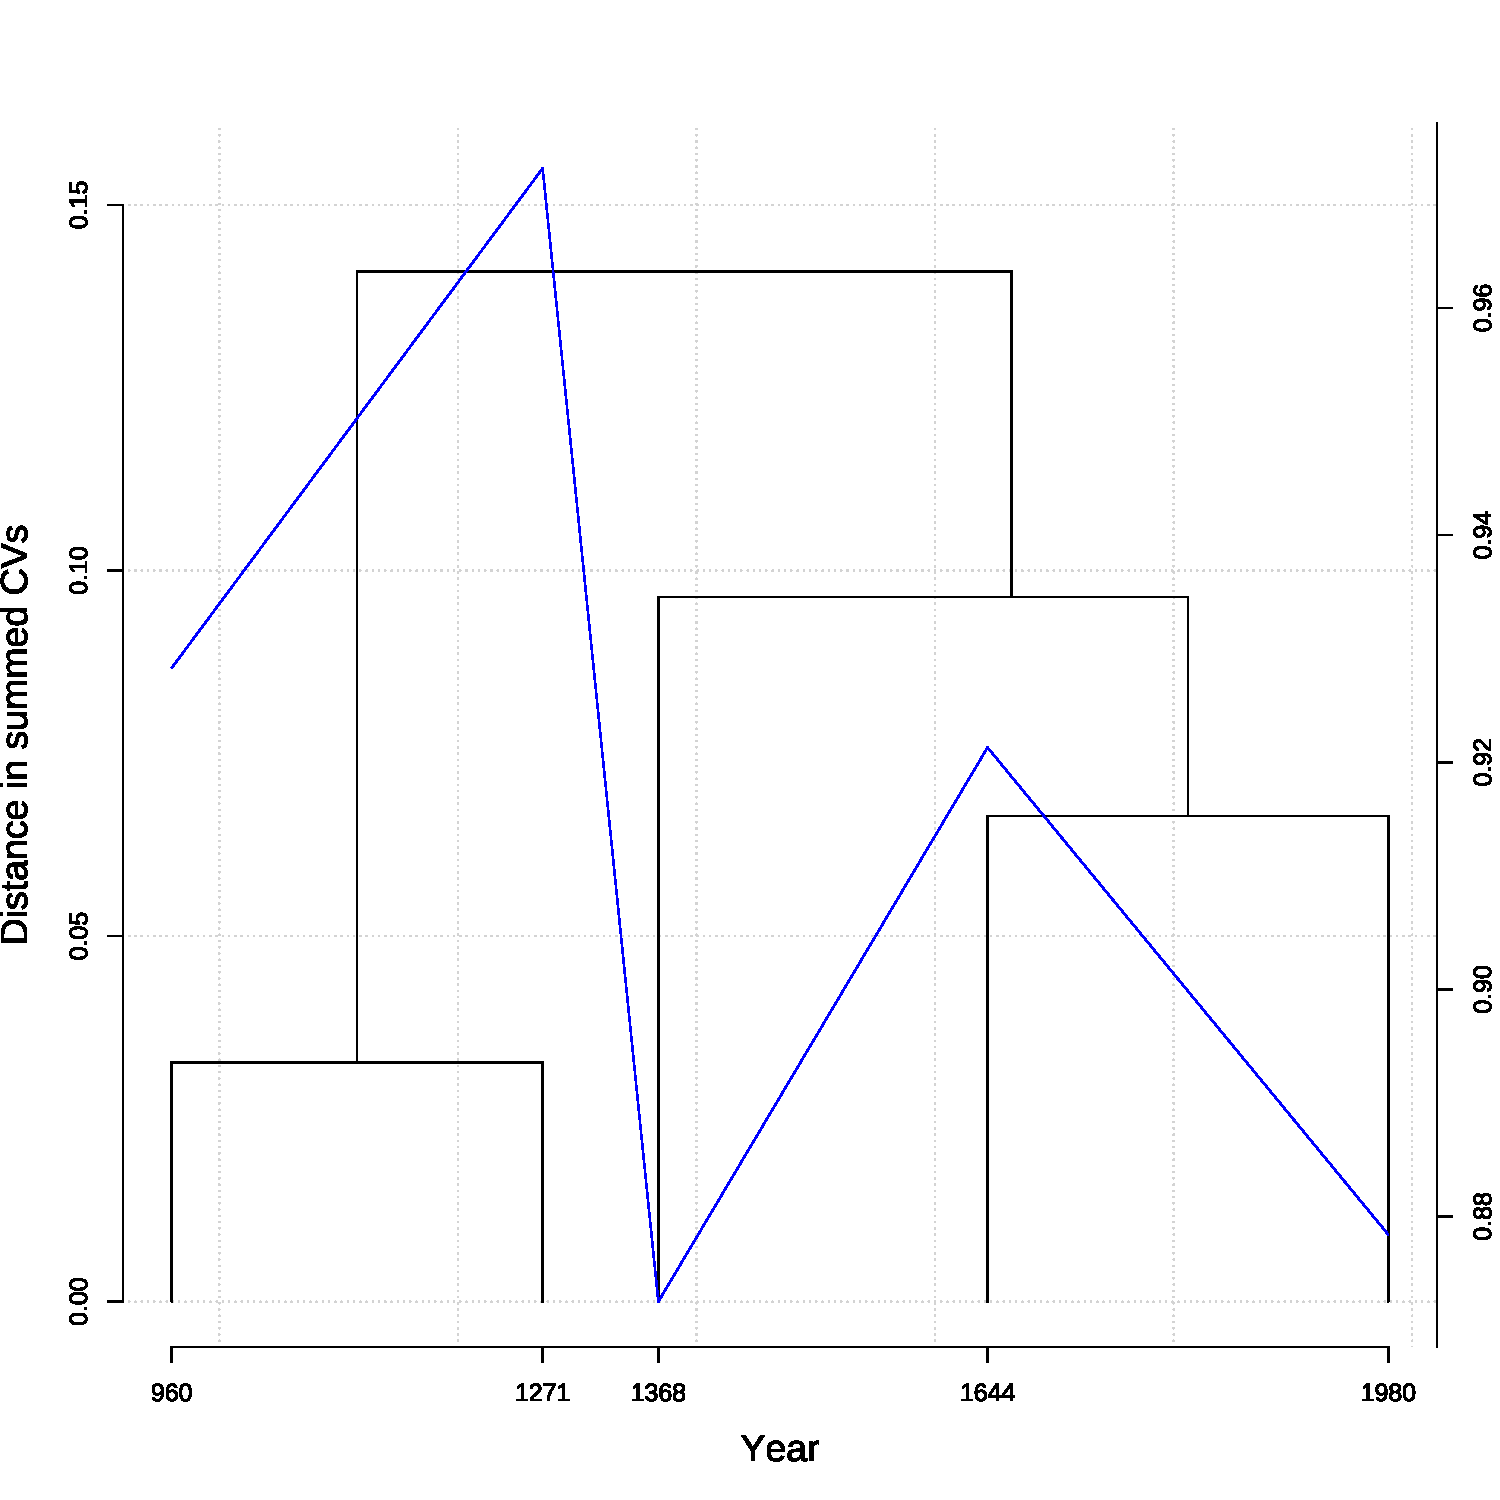
\includegraphics[width=\linewidth]{figures_new/measures/VNC_measure_dist_w1_first_embed.pdf}
    \caption*{1\sts  , ws=1}
  \end{subfigure}
  \quad
  \begin{subfigure}{0.3\textwidth}
    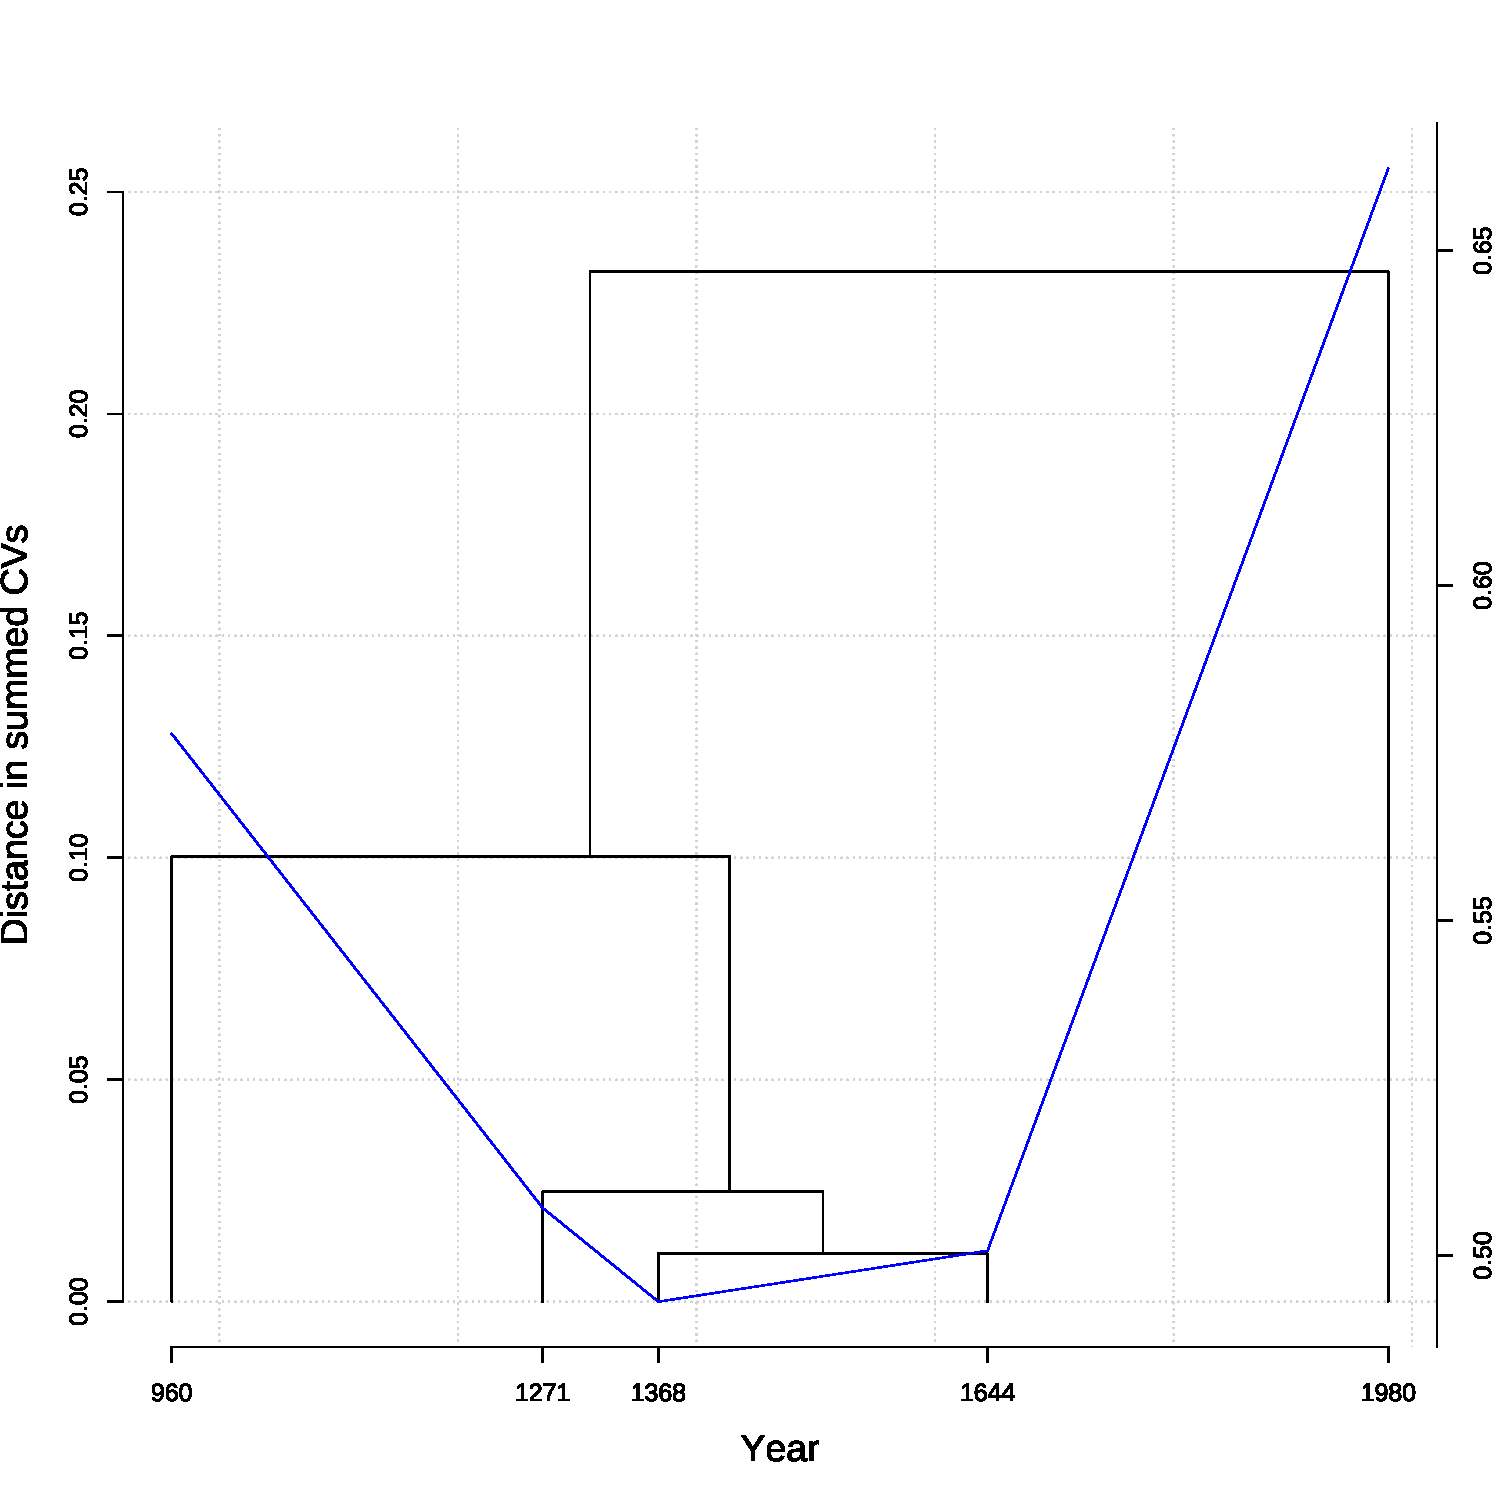
\includegraphics[width=\linewidth]{figures_new/measures/VNC_measure_dist_w1_second_embed_global.pdf}
    \caption*{2\nds  (global), ws=1}
  \end{subfigure}
  \quad
  \begin{subfigure}{0.3\textwidth}
    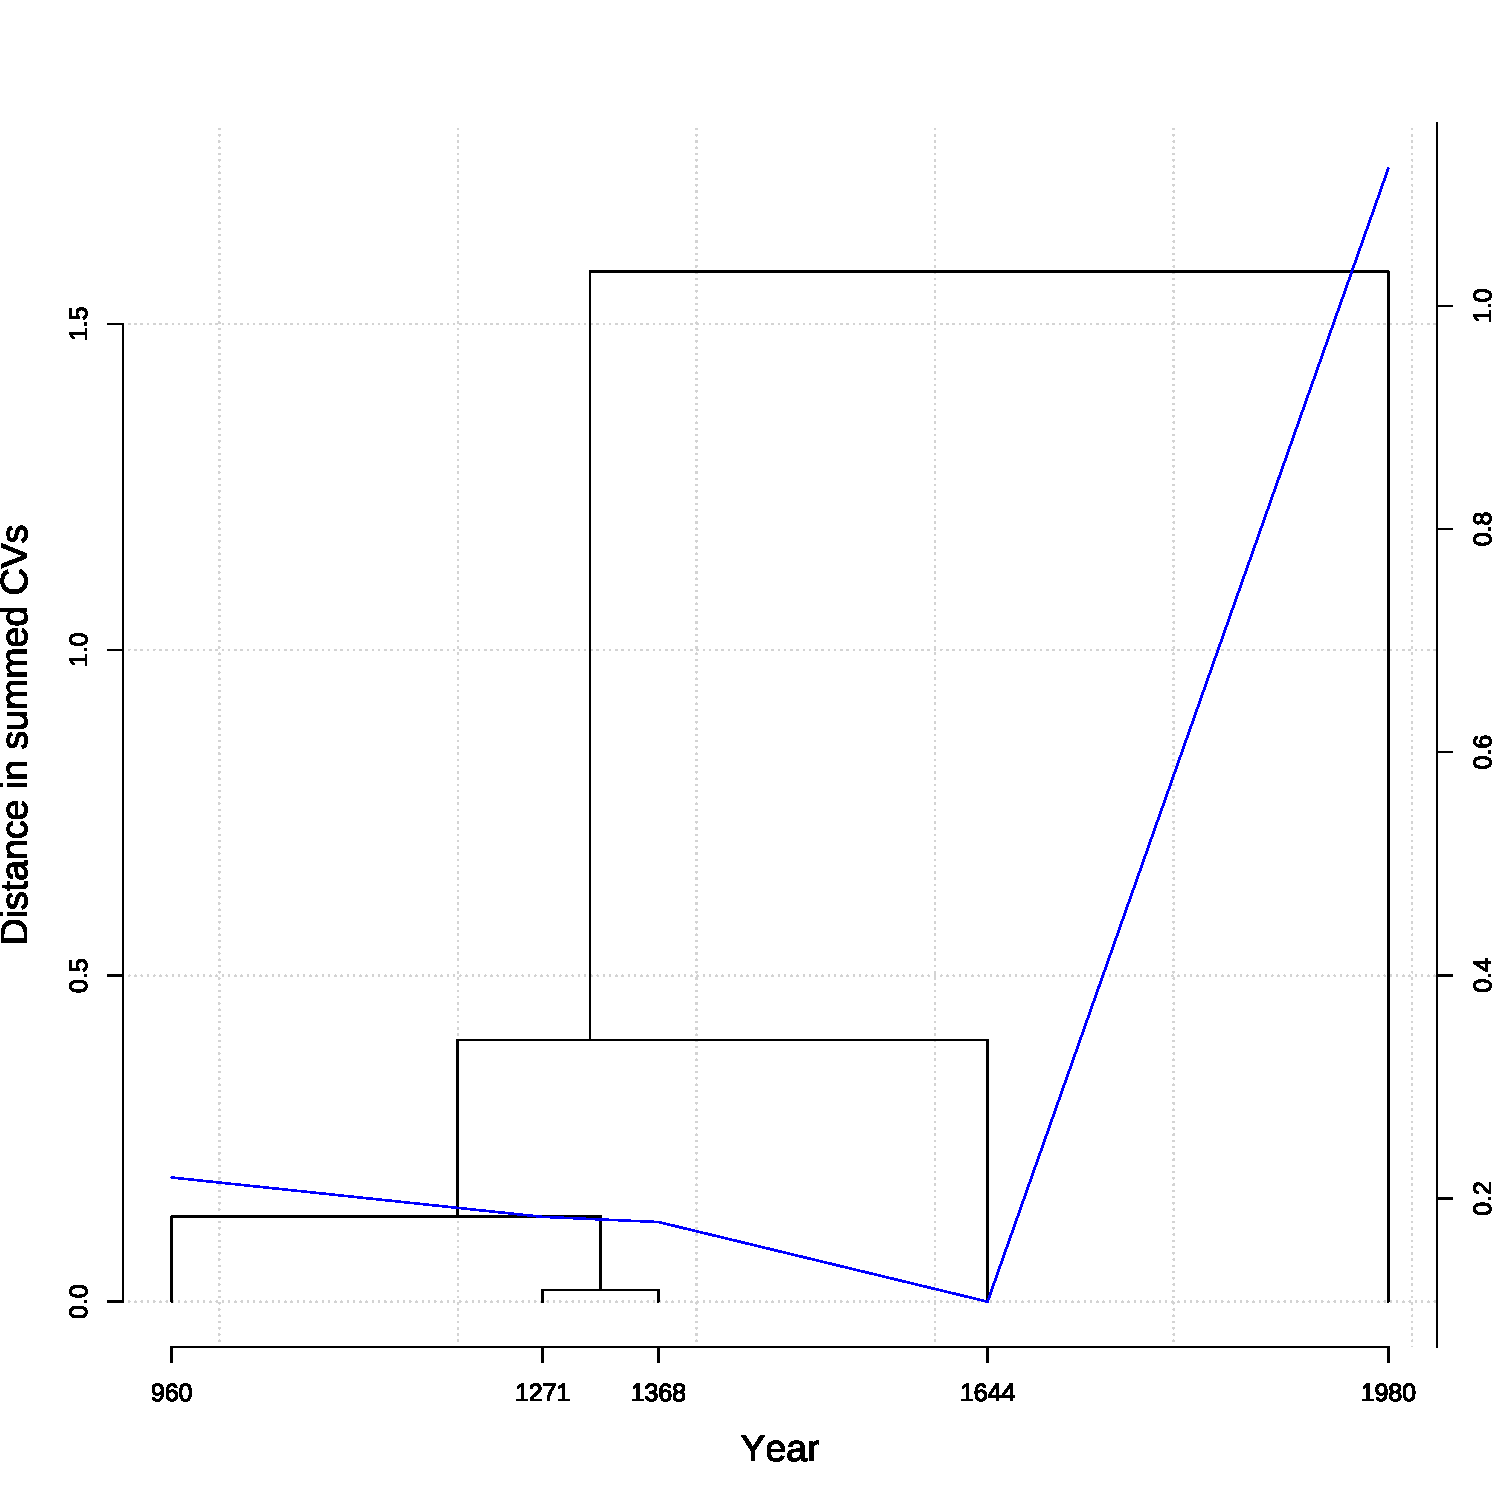
\includegraphics[width=\linewidth]{figures_new/measures/VNC_measure_dist_w1_second_embed_local.pdf}
    \caption*{2\nds  (local), ws=1}
  \end{subfigure}
  
  \medskip
  \begin{subfigure}{0.3\textwidth}
    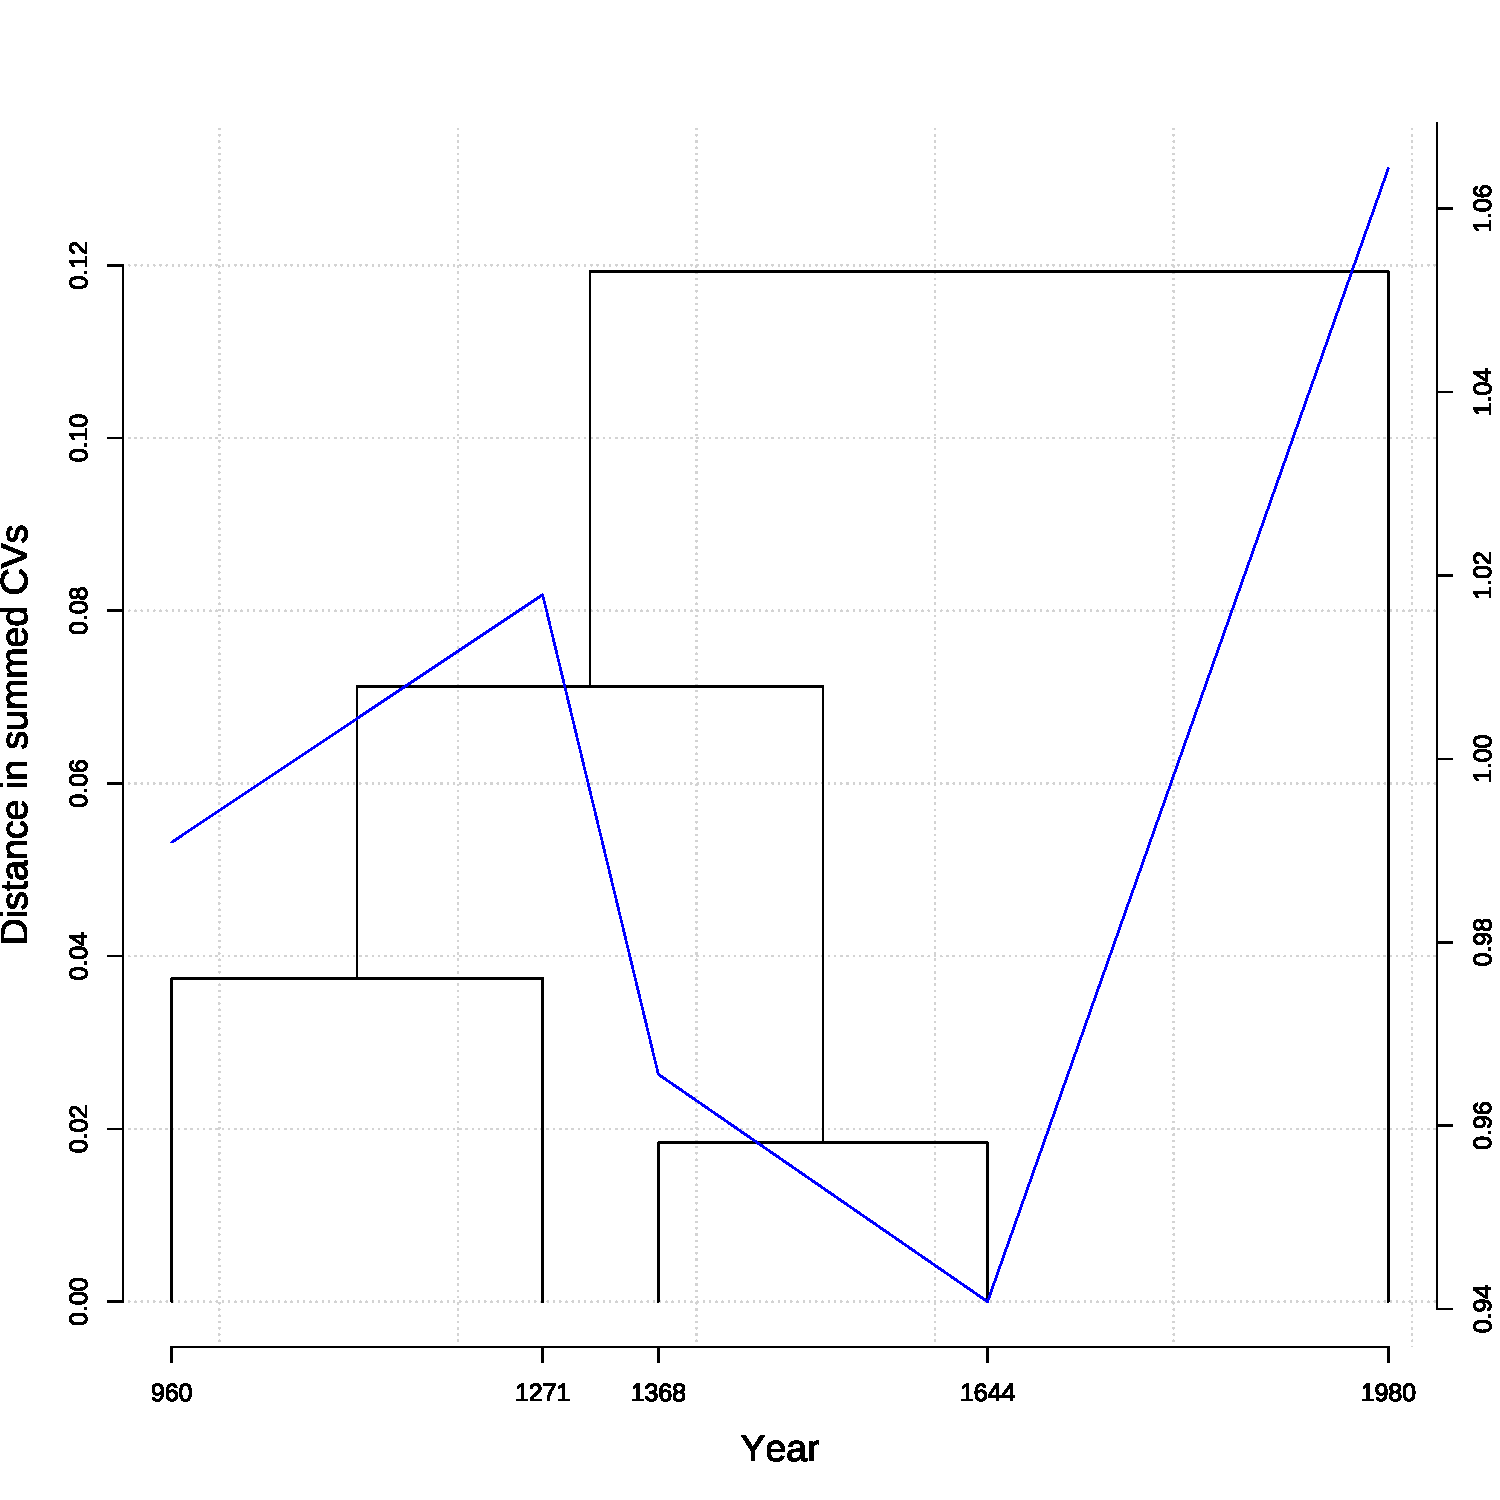
\includegraphics[width=\linewidth]{figures_new/measures/VNC_measure_dist_w5_first_embed.pdf}
    \caption*{1\sts  , ws=5}
  \end{subfigure}
  \quad
  \begin{subfigure}{0.3\textwidth}
    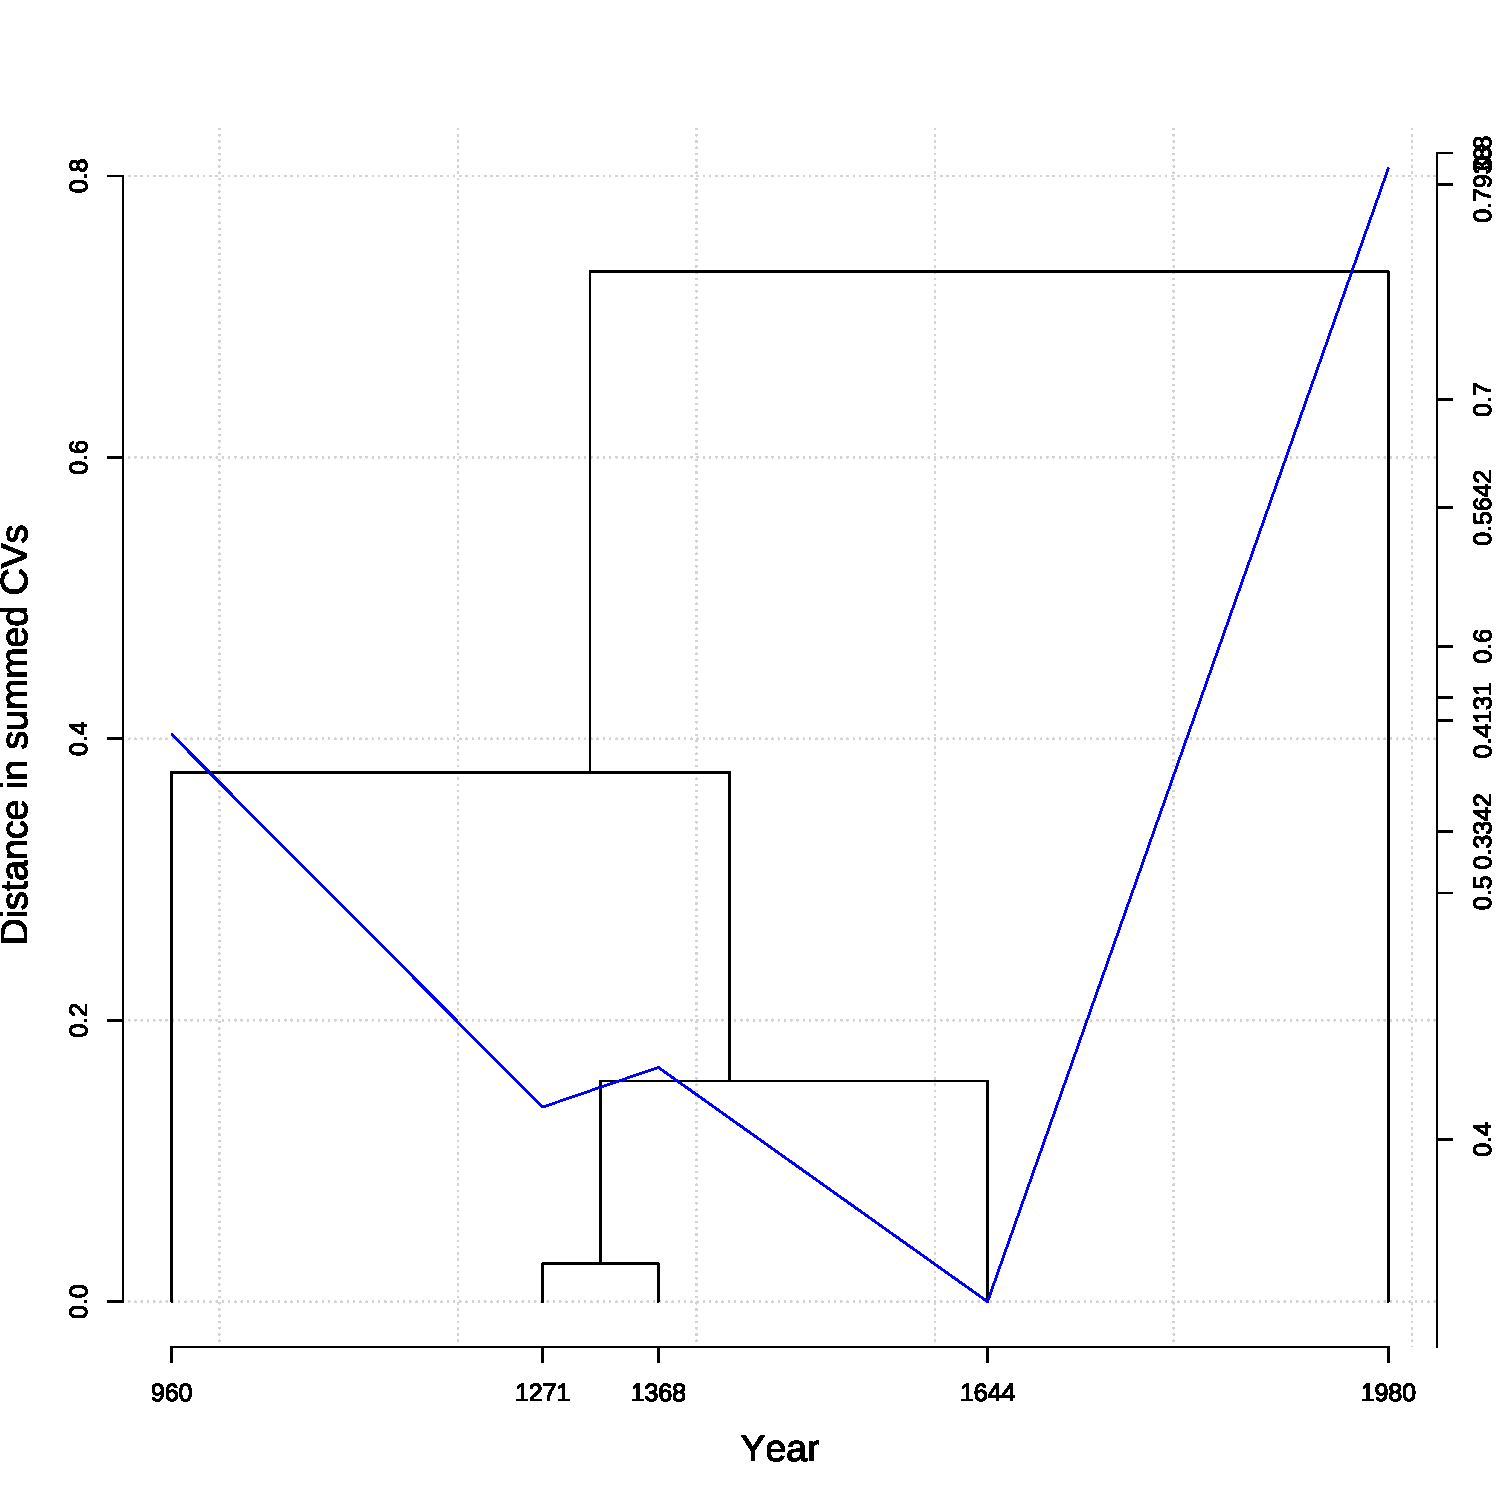
\includegraphics[width=\linewidth]{figures_new/measures/VNC_measure_dist_w5_second_embed_global.pdf}
    \caption*{2\nds  (global), ws=5}
  \end{subfigure}
  \quad
  \begin{subfigure}{0.3\textwidth}
    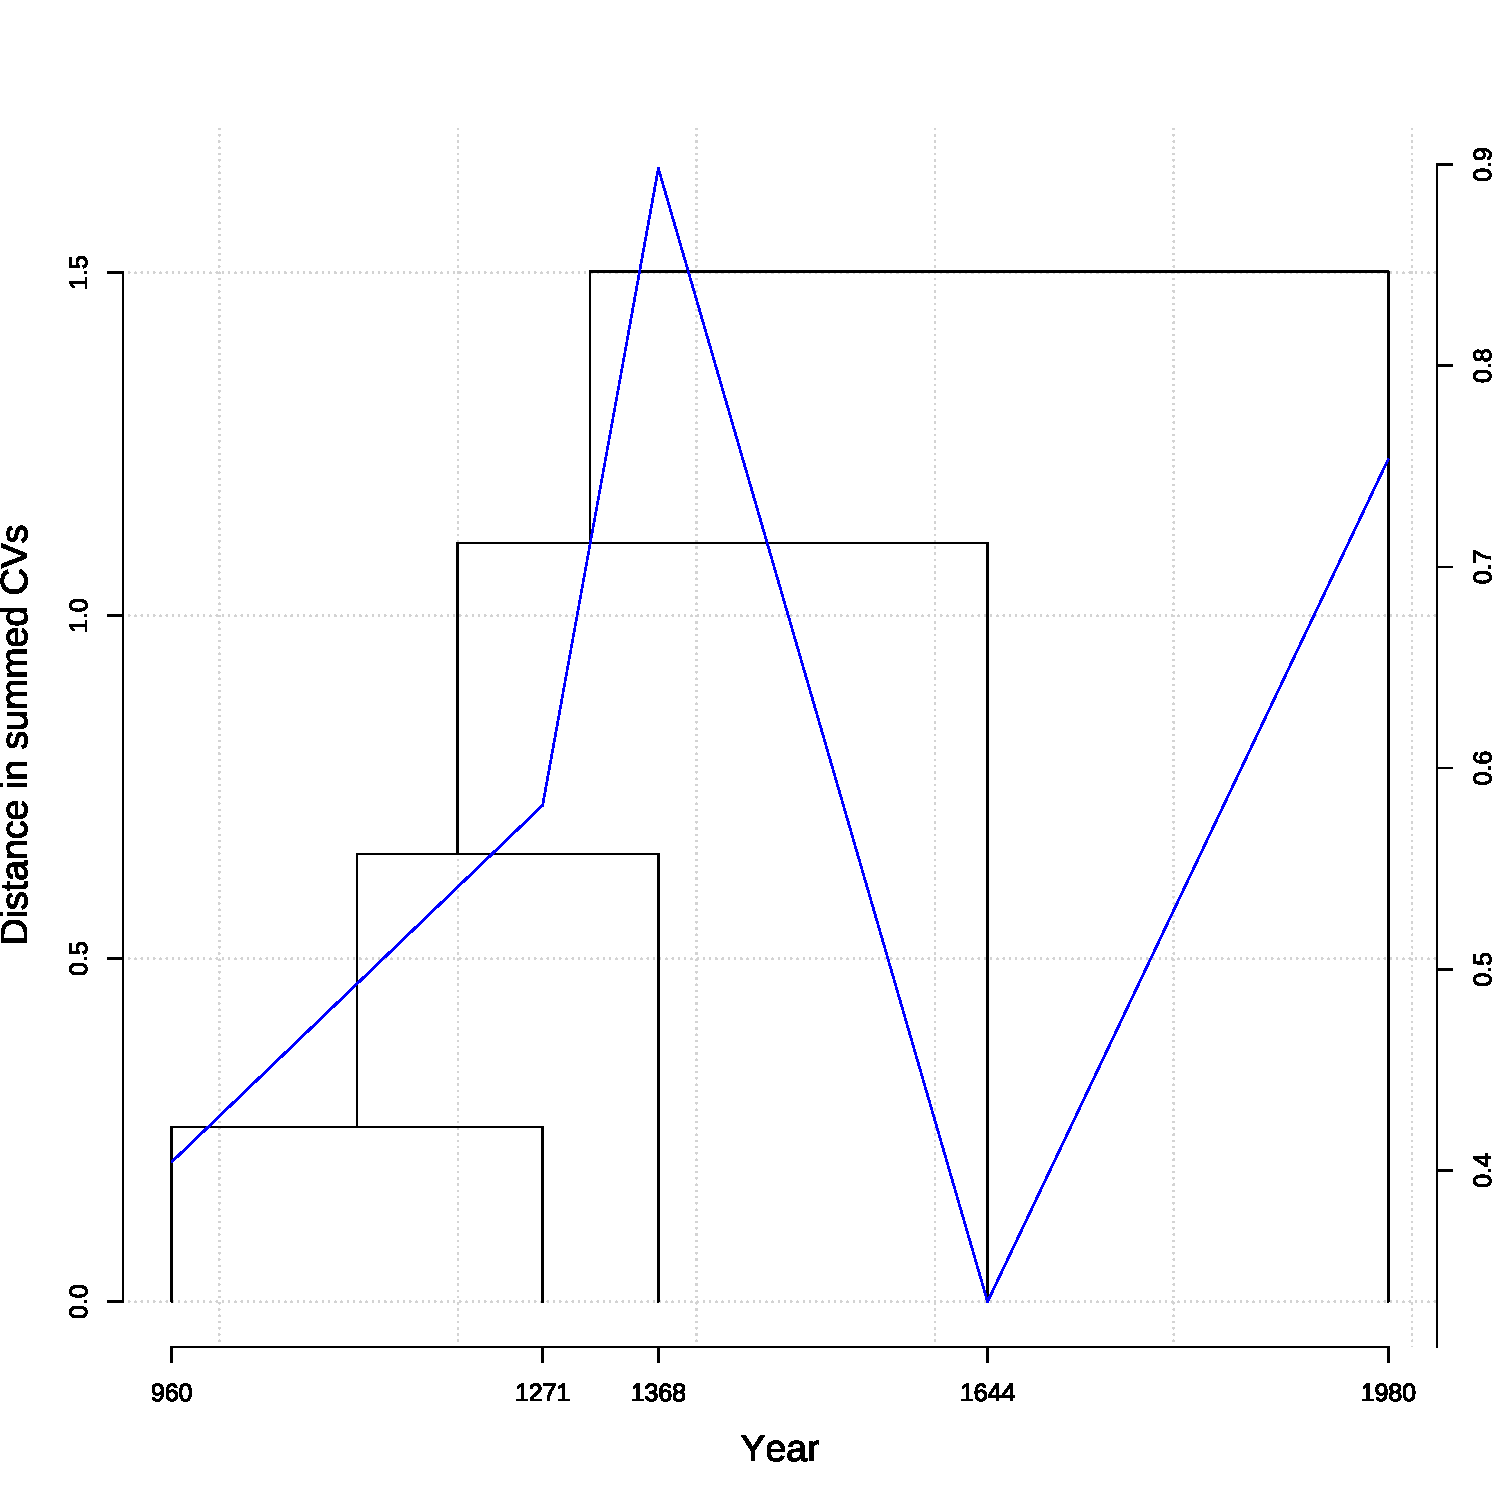
\includegraphics[width=\linewidth]{figures_new/measures/VNC_measure_dist_w5_second_embed_local.pdf}
    \caption*{2\nds  (local), ws=5}
  \end{subfigure}
  
  \medskip
  \begin{subfigure}{0.3\textwidth}
    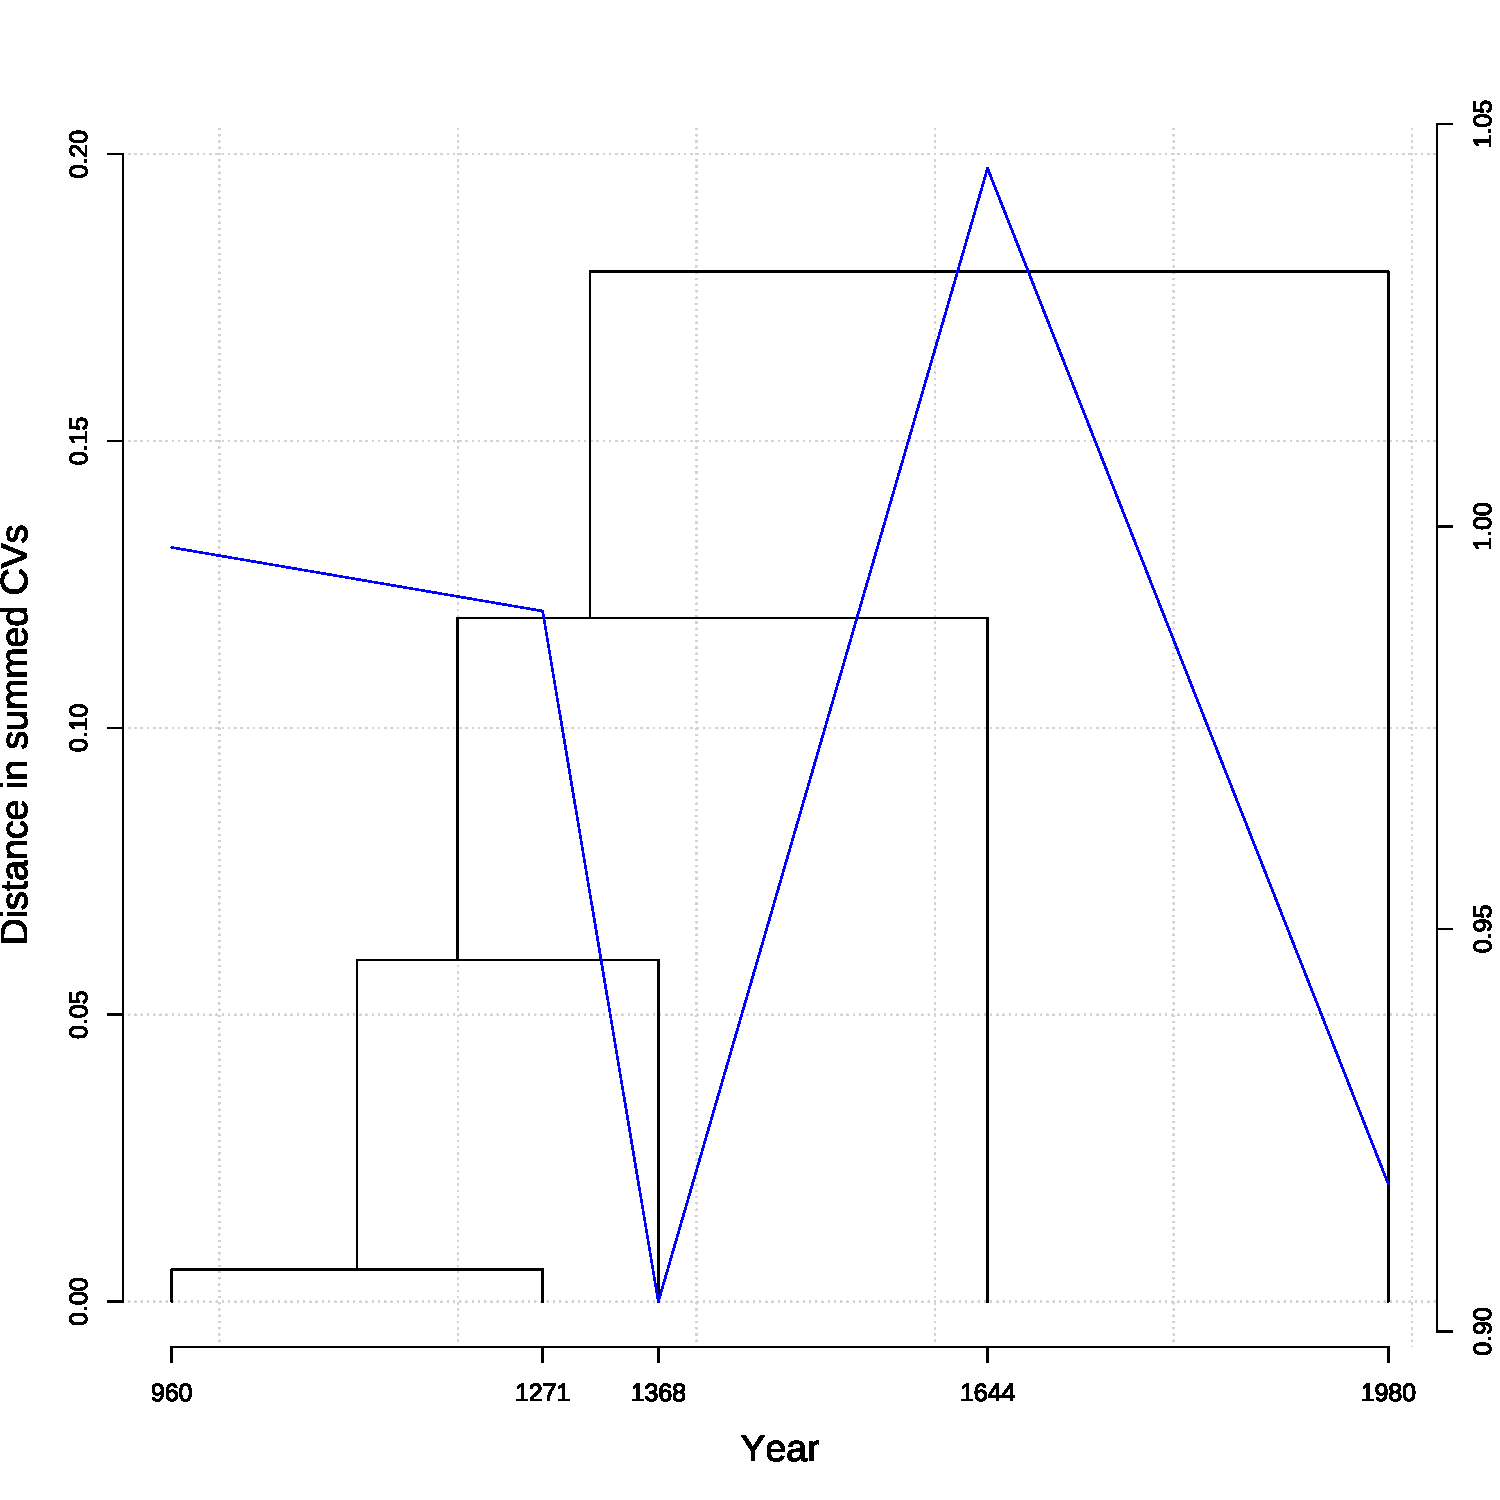
\includegraphics[width=\linewidth]{figures_new/measures/VNC_measure_dist_w10_first_embed.pdf}
    \caption*{1\sts  , ws=10}
  \end{subfigure}
  \quad
  \begin{subfigure}{0.3\textwidth}
    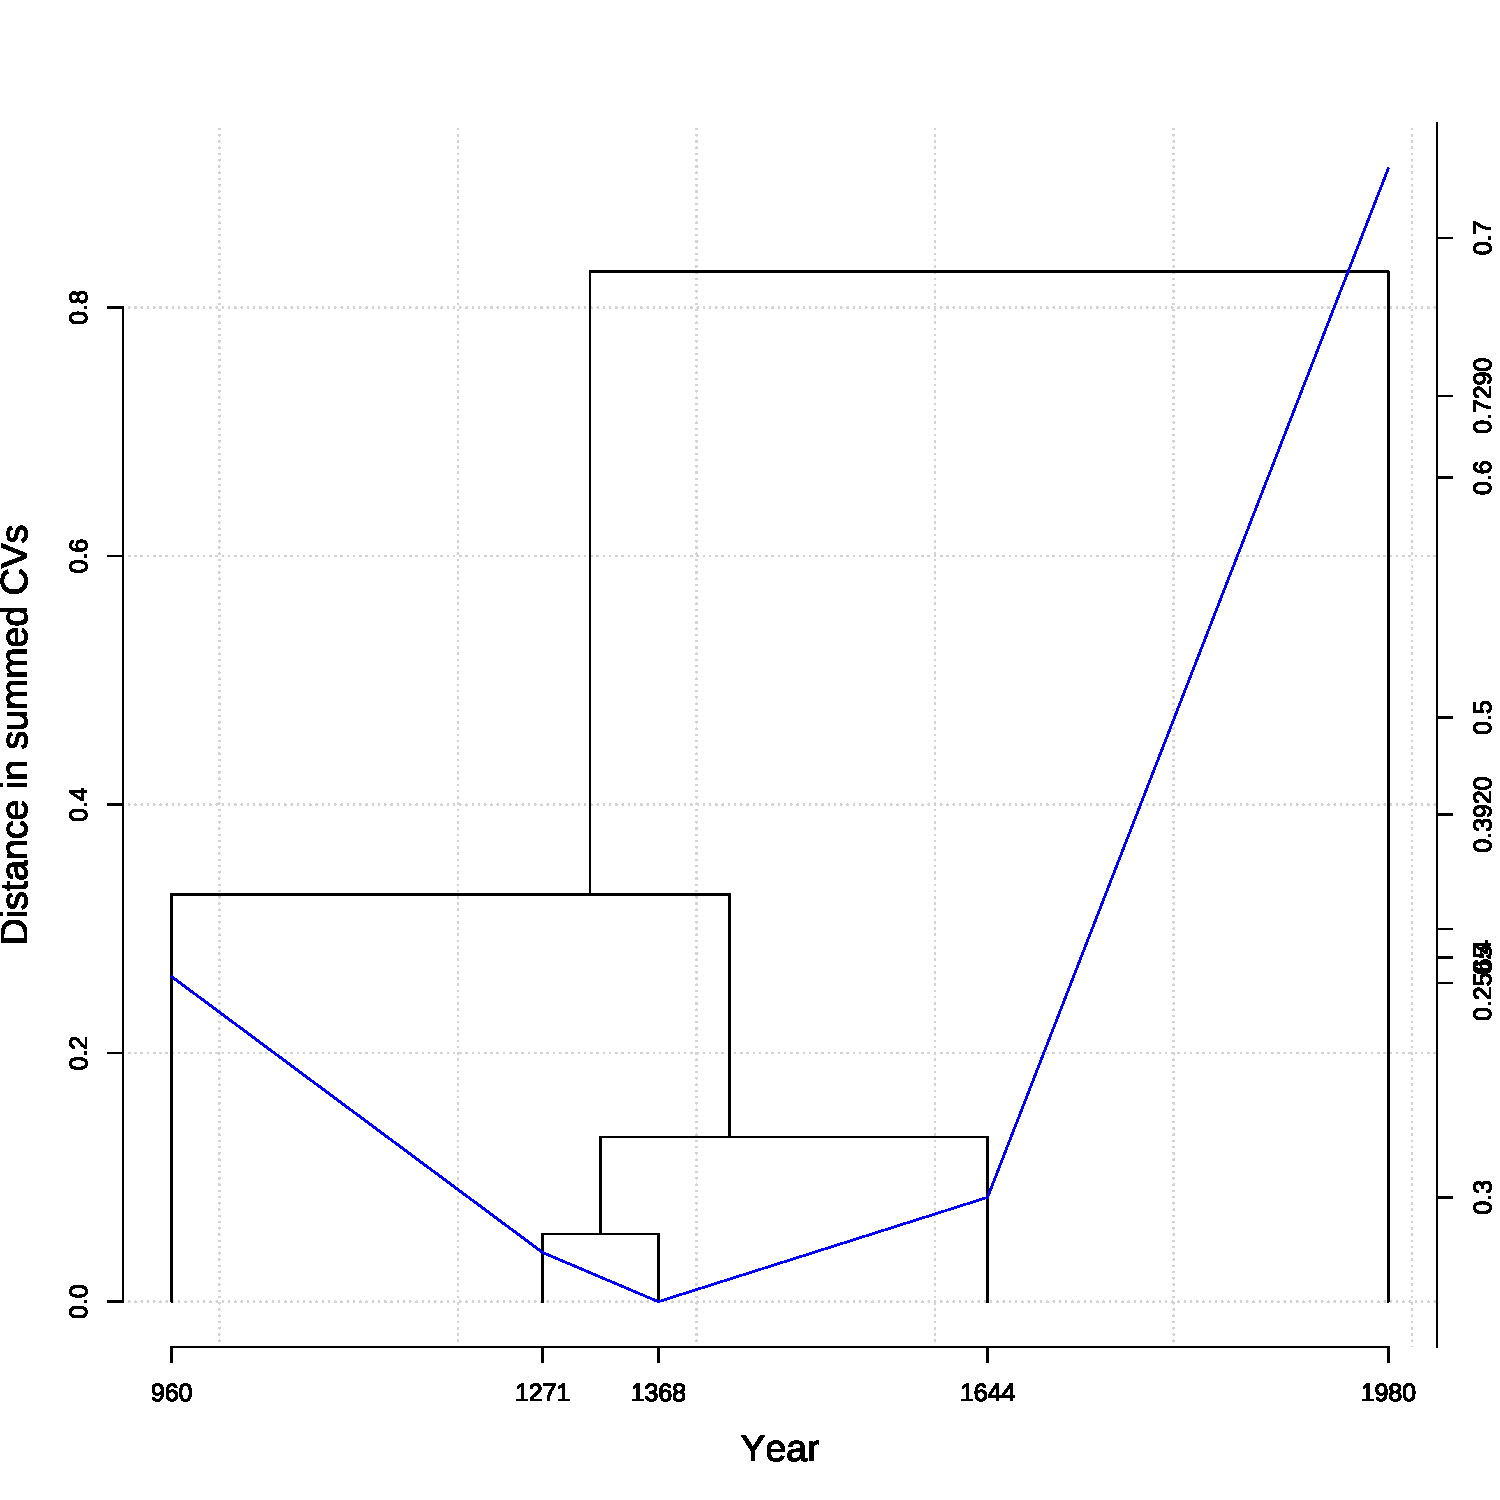
\includegraphics[width=\linewidth]{figures_new/measures/VNC_measure_dist_w10_second_embed_global.pdf}
    \caption*{2\nds  (global), ws=10}
  \end{subfigure}
  \quad
  \begin{subfigure}{0.3\textwidth}
    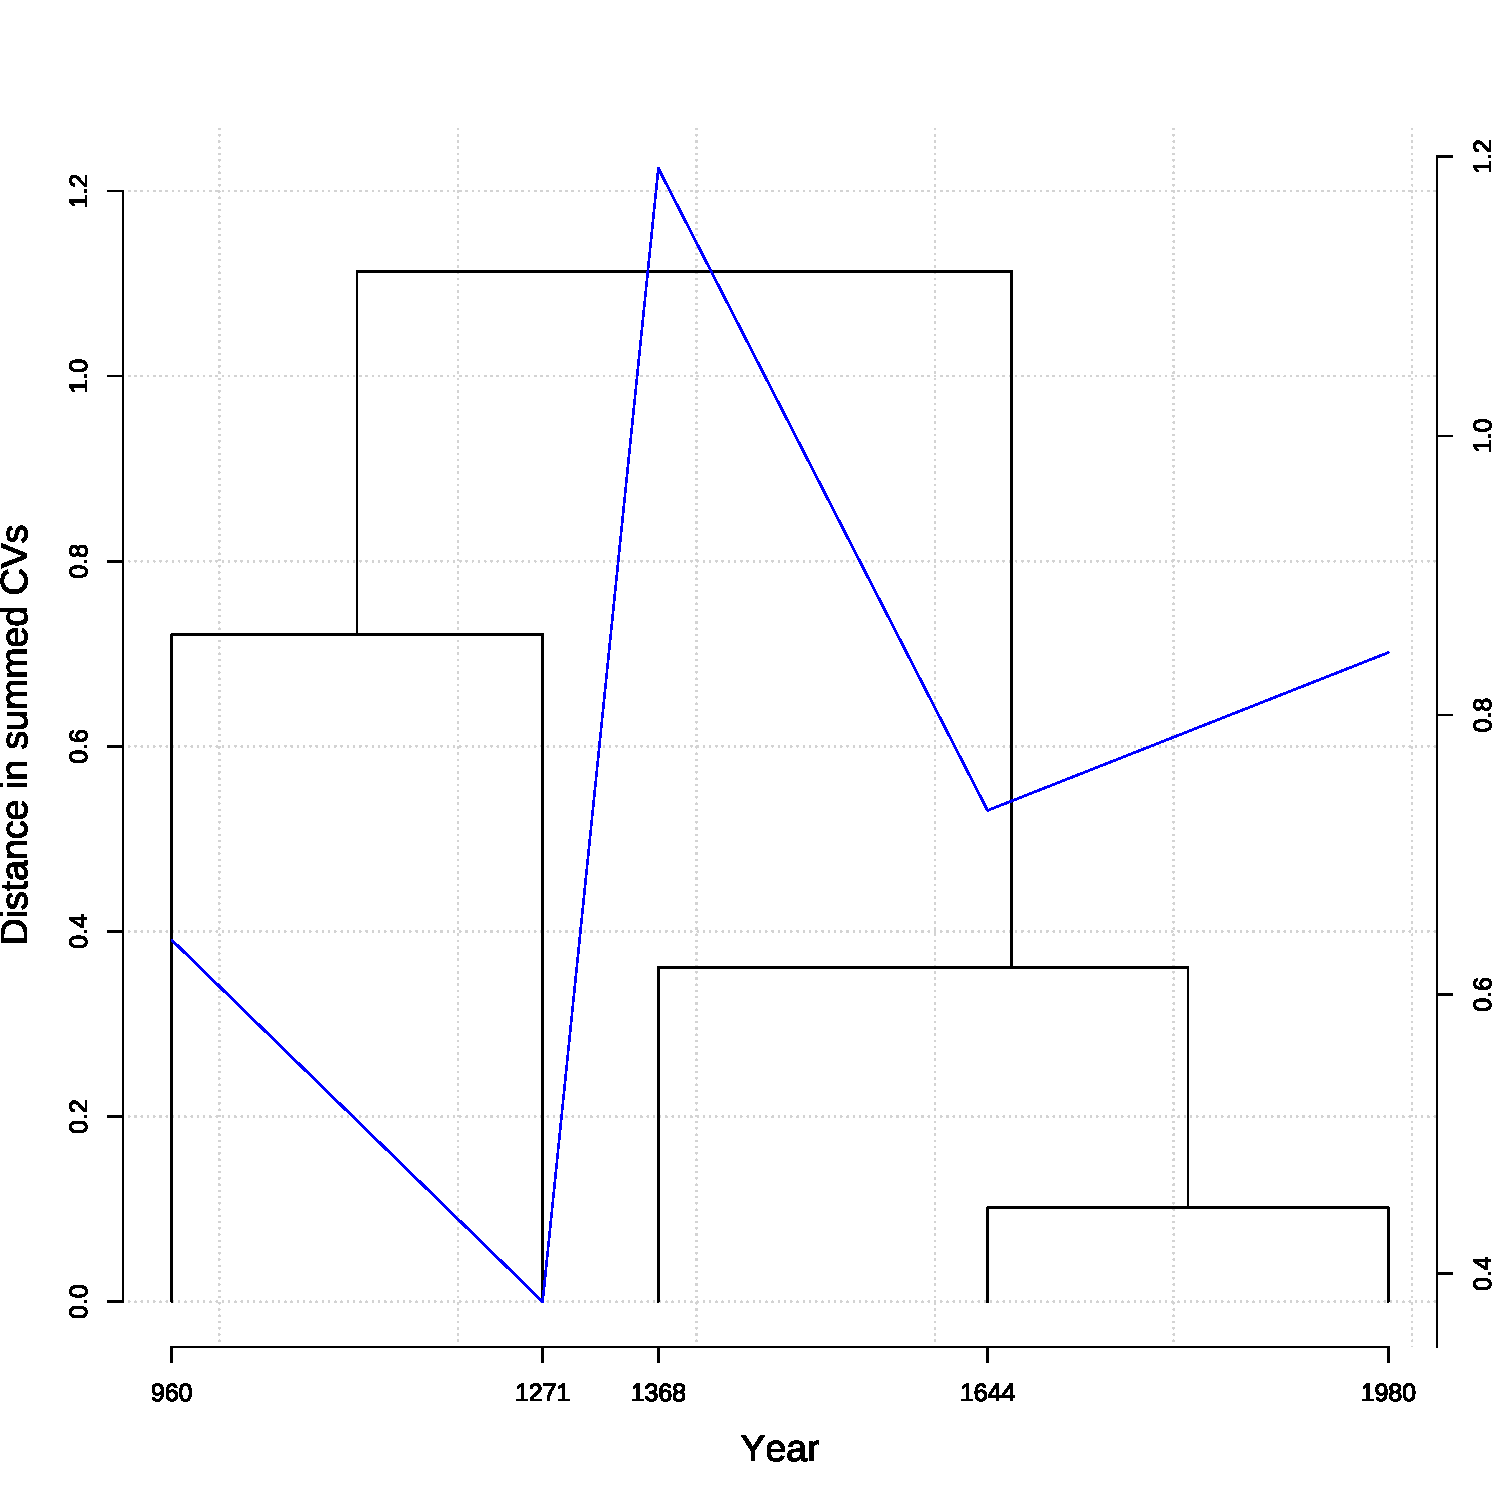
\includegraphics[width=\linewidth]{figures_new/measures/VNC_measure_dist_w10_second_embed_local.pdf}
    \caption*{2\nds  (local), ws=10}
  \end{subfigure}
  
  \caption{Results of VNC periodization of global and local measures of semantic change for \jia}
\end{figure}

\begin{figure}[H]
  \centering
  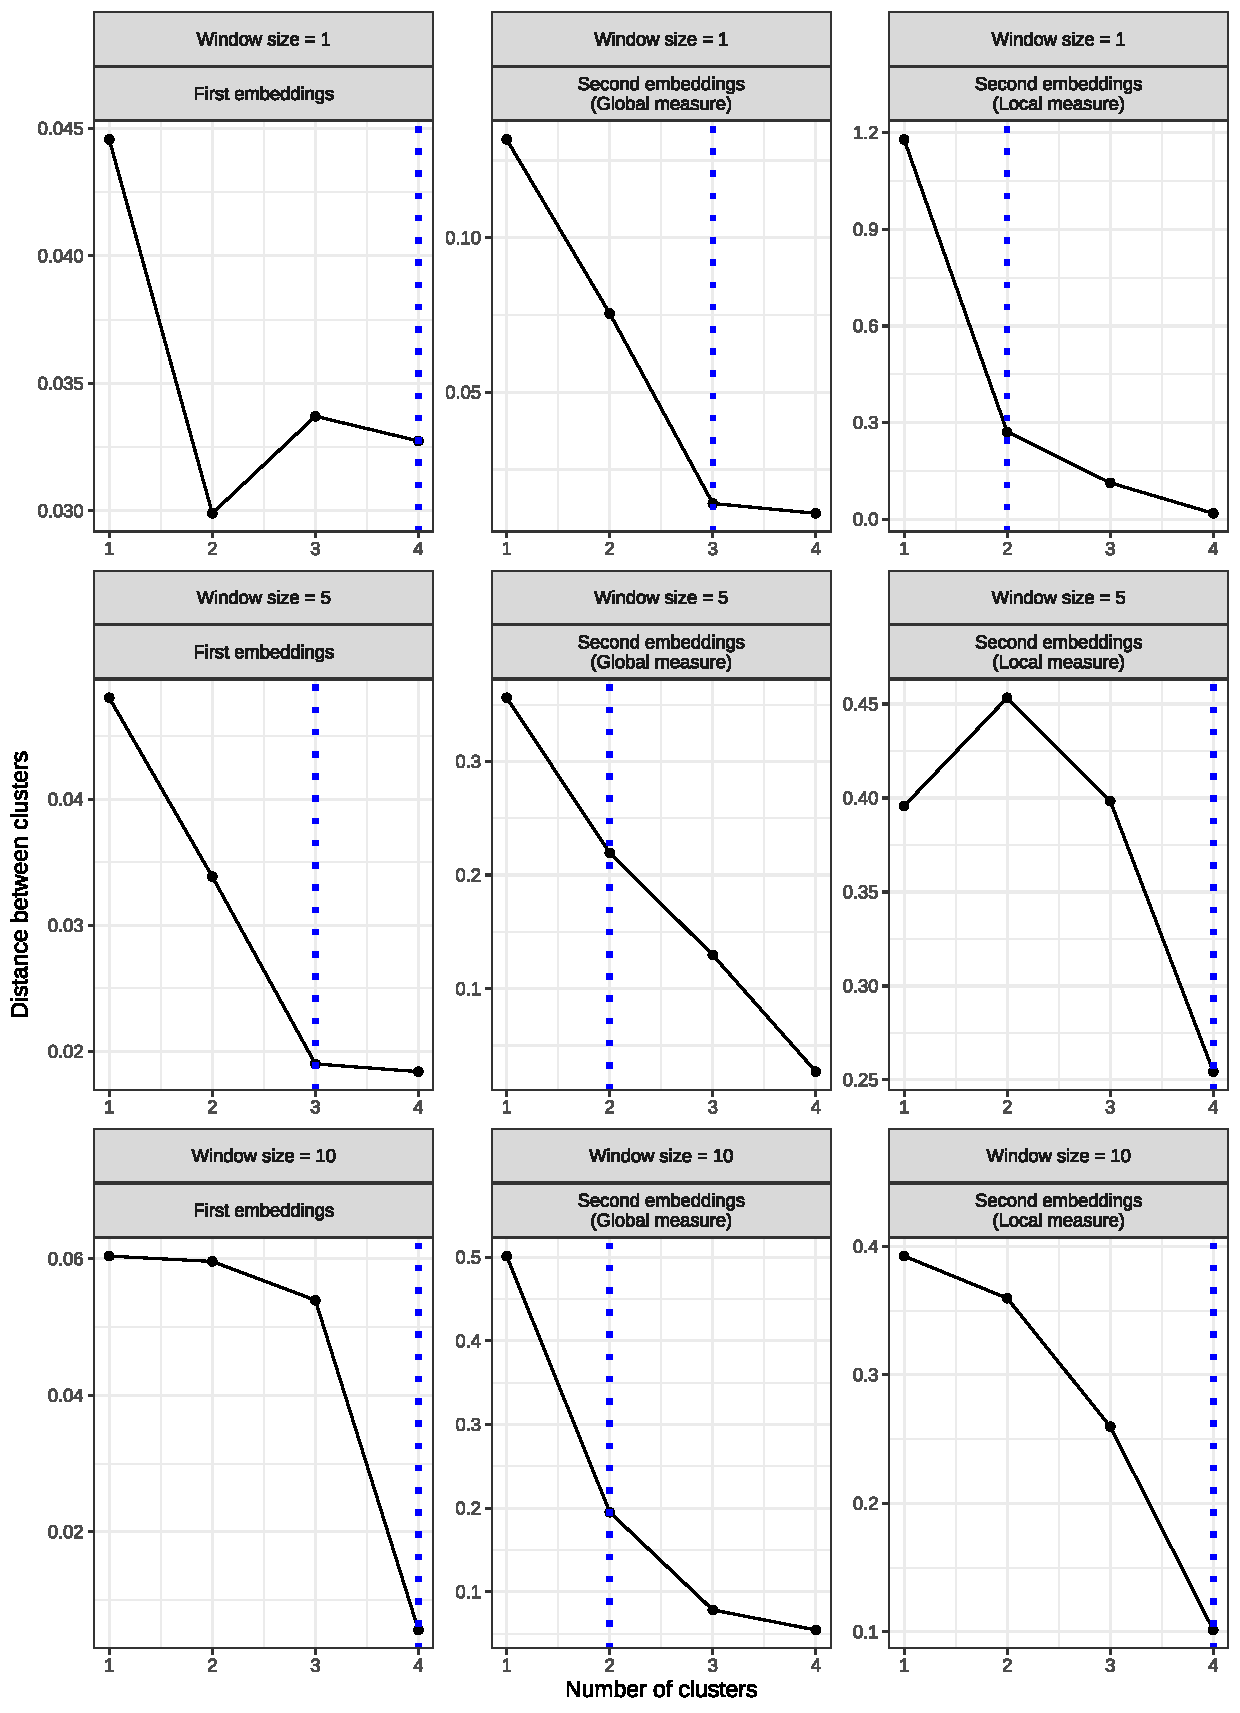
\includegraphics[width=0.95\textwidth]{figures_new/measures/screeplot.pdf}
  \caption{Screeplot of VNC periodization of global and local measures of semantic change for \jia}
\end{figure}

\end{document}